\documentclass[a4paper, 11pt]{article}

\usepackage[T1]{fontenc}
\usepackage[utf8]{inputenc}

\usepackage{csquotes}
\usepackage{pgfgantt}

\usepackage[french]{babel}
\usepackage[toc]{glossaries}
\usepackage{listings}
\usepackage{xcolor}
\usepackage[table]{xcolor}
\usepackage{float}
\usepackage{tabularx}
\usepackage{pgfplots}
\usepackage[colorlinks=true, linkcolor=blue, urlcolor=cyan, citecolor=green]{hyperref}


\usepackage{titlesec}
\setcounter{secnumdepth}{4} % numéroter jusqu'à \paragraph (niveau 4)
\setcounter{tocdepth}{4}    % inclure jusqu'à \paragraph dans la table des matières

% Rendre \paragraph visible comme un titre de niveau 4 (bloc, non run-in)
\titleformat{\paragraph}[block]{\normalfont\bfseries}{\theparagraph}{1em}{}
\titlespacing*{\paragraph}{0pt}{3.5ex plus 1ex minus .2ex}{1ex}


\pgfplotsset{compat=1.17}


\definecolor{darkblue}{RGB}{31, 73, 125}
\definecolor{medblue}{RGB}{68, 114, 196}
\definecolor{lightblue}{RGB}{189, 215, 238}
\definecolor{lightgreen}{RGB}{169, 208, 142}


\definecolor{backgray}{rgb}{0.15,0.15,0.15} % Fond gris très foncé
\definecolor{codegray}{rgb}{0.6,0.6,0.6}    % Commentaires gris clair
\definecolor{keywordblue}{rgb}{0.4,0.8,1.0} % Mots-clés bleu clair
\definecolor{stringgreen}{rgb}{0.5,1.0,0.5} % Chaînes vert pâle
\definecolor{textwhite}{rgb}{0.95,0.95,0.95} % Texte principal presque blanc
\definecolor{codebg}{RGB}{248,248,248}
\definecolor{linenumber}{RGB}{150,150,150}
\definecolor{keywordpurple}{RGB}{180,0,255}
\definecolor{stringgreen}{RGB}{0,128,0}
\definecolor{bordergray}{RGB}{220,220,220}


\definecolor{bluelight}{RGB}{210, 228, 245}
\definecolor{blueborder}{RGB}{70, 130, 180}
\definecolor{greybox}{RGB}{230, 228, 220}
\definecolor{greyborder}{RGB}{160, 155, 140}
\definecolor{bluetext}{RGB}{70, 130, 180}
\definecolor{dashedborder}{RGB}{140, 140, 140}

\definecolor{gh-keyword}{HTML}{CF222E}   % rouge pour les clés YAML



 
% ── Palette ──────────────────────────────────────────────────────────────────
\definecolor{netblue}{RGB}{30,  80, 160}
\definecolor{firered}{RGB}{180,  30,  30}
\definecolor{swgreen}{RGB}{ 34, 120,  60}
\definecolor{devpurp}{RGB}{ 90,  50, 150}
\definecolor{srvoran}{RGB}{190, 100,  10}
\definecolor{voiptel}{RGB}{ 10, 130, 150}
\definecolor{wificolor}{RGB}{ 70, 140, 200}
\definecolor{boxbg}  {RGB}{240, 245, 255}
\definecolor{zonebg} {RGB}{230, 238, 252}
\definecolor{servbg} {RGB}{255, 245, 230}
\definecolor{devbg}  {RGB}{240, 232, 255}
\definecolor{voipbg} {RGB}{225, 248, 250}
\definecolor{wifibg} {RGB}{232, 242, 255}
\definecolor{extbg}  {RGB}{235, 235, 235}

\tikzset{
  dev/.style={
    rectangle, rounded corners=5pt,
    draw=#1!70!black, fill=#1!10,
    font=\sffamily\scriptsize, text width=3.0cm, align=left,
    inner sep=5pt, minimum height=1.2cm,
    drop shadow={shadow xshift=.6pt, shadow yshift=-.6pt, opacity=.2}
  },
  internet/.style={
    ellipse, draw=netblue, fill=netblue!10,
    font=\sffamily\small\bfseries,
    minimum width=2.4cm, minimum height=1.0cm,
    drop shadow={shadow xshift=.6pt, shadow yshift=-.6pt, opacity=.2}
  },
  zonetitle/.style={font=\sffamily\tiny\bfseries, text=#1},
  netlink/.style ={draw=#1, line width=1.3pt, -{Stealth[length=4pt]}, rounded corners=3pt},
  netbidi/.style ={draw=#1, line width=1.3pt,
    {Stealth[length=4pt]}-{Stealth[length=4pt]}, rounded corners=3pt},
}

\tikzset{
  boxdark/.style={
    rectangle, rounded corners=4pt,
    fill=darkblue, draw=darkblue,
    text=white, font=\small\bfseries,
    text width=3.2cm, align=center,
    minimum height=1.1cm, inner sep=6pt
  },
  boxmed/.style={
    rectangle, rounded corners=4pt,
    fill=medblue, draw=medblue,
    text=white, font=\small\bfseries,
    text width=3.2cm, align=center,
    minimum height=1.1cm, inner sep=6pt
  },
  boxlight/.style={
    rectangle, rounded corners=4pt,
    fill=lightblue, draw=lightblue,
    text=black, font=\small,
    text width=3.2cm, align=center,
    minimum height=1.1cm, inner sep=6pt
  },
  boxgreen/.style={
    rectangle, rounded corners=4pt,
    fill=lightgreen, draw=lightgreen,
    text=black, font=\small,
    text width=3.2cm, align=center,
    minimum height=1.1cm, inner sep=6pt
  },
  line/.style={draw=gray!70, thick}
}

\lstdefinelanguage{WazuhXML}{
    language=XML,
    morekeywords={
        decoder,
        prematch,
        regex,
        order,
        parent,
        plugin_decoder,
        group,
        rule,
        if_sid,
        list,
        description,
        known-devices,
    },
    keywordstyle=\color{keywordpurple}\bfseries,
    morestring=[b]",
    stringstyle=\color{stringgreen}
}

\lstdefinelanguage{customXML}{
  basicstyle=\color{red}\ttfamily\small,
  sensitive=true,
  % Comments in green
  morecomment=[s]{<!--}{-->},
  commentstyle=\color{green},
  % Tag names in blue (inside <...>)
  moredelim=**[is][\color{blue}]{\<}{\>},
  % Keep regular text in red (default)
}

\lstdefinelanguage{ScaYAML}{
    keywords={
        id, title, description, rationale, remediation,
        compliance, condition, rules, profile, check,
        cis, cis_csc, hipaa, gdpr_IV, tsc, all, any, none
    },
    keywordstyle=\color{keywordpurple}\bfseries,
    morestring=[b]",
    morestring=[b]',
    stringstyle=\color{stringgreen},
    morecomment=[l]{\#},
    commentstyle=\color{codegray}\itshape,
    sensitive=true,
}


\lstset{
    backgroundcolor=\color{codebg},
    basicstyle=\ttfamily\small\color{black},
    keywordstyle=\color{keywordpurple},
    stringstyle=\color{stringgreen},
    commentstyle=\color{gray}\itshape,
    numbers=left,
    numberstyle=\tiny\color{linenumber},
    numbersep=10pt,
    frame=single,
    rulecolor=\color{bordergray},
    breaklines=true,
    showstringspaces=false,
    tabsize=2,
    xleftmargin=5pt,
    framexleftmargin=5pt
}




%Pour la création d'un glossaire, il faut mettre toutes les entrées dans le préambule
\newglossaryentry{ANSSI}{
   name={ANSSI},
   description={Agence nationale de la sécurité des systèmes d'information}}
\newglossaryentry{RSSI}{
   name={RSSI},
   description={Responsable de la sécurité des systèmes d'information, chargé de la mise en œuvre de la politique de sécurité au sein d'une organisation}}
\newglossaryentry{Deep Learning}{
   name={Deep Learning},
   description={Sous-domaine de l'apprentissage automatique qui utilise des réseaux de neurones profonds pour modéliser des données complexes et extraire des caractéristiques hiérarchiques}}
\newglossaryentry{CVE}{
   name={CVE},
    description={Common Vulnerabilities and Exposures, un système de référence pour les vulnérabilités de sécurité connues dans les logiciels et les systèmes informatiques}}
\newglossaryentry{CVSS}{
   name={CVSS},
    description={Common Vulnerability Scoring System, un cadre standardisé pour évaluer la gravité des vulnérabilités de sécurité dans les systèmes informatiques}}
\newglossaryentry{CIS Benchmarks}{
   name={CIS Benchmarks},
   description={Center for Internet Security Benchmarks, ensemble de bonnes pratiques de sécurité pour la configuration des systèmes d'exploitation et des applications}}
\newglossaryentry{GPO}{
   name={GPO},
   description={Group Policy Object, mécanisme de stratégies de groupe permettant de configurer et de sécuriser les postes et utilisateurs d’un domaine Active Directory}
}
\newglossaryentry{SIEM}{
   name={SIEM},
   description={Security Information and Event Management, solution centralisant et corrélant les événements de sécurité afin de détecter les incidents et améliorer la visibilité du SI}
}
\newglossaryentry{DNS}{
   name={DNS},
   description={Domain Name System, service permettant la résolution des noms de domaine en adresses IP, indispensable au fonctionnement d’Active Directory}
}

\newglossaryentry{DHCP}{
   name={DHCP},
   description={Dynamic Host Configuration Protocol, service permettant l’attribution automatique des paramètres réseau aux postes clients}
}
\newglossaryentry{Hyperviseur de type 1}{
   name={Hyperviseur de type 1},
   description={Hyperviseur fonctionnant directement sur le matériel, sans système d’exploitation hôte, offrant de meilleures performances et une sécurité accrue}
}
\newglossaryentry{VLAN}{
   name={VLAN},
   description={Virtual Local Area Network, technique de segmentation réseau permettant d’isoler logiquement des flux et d’améliorer la sécurité}
}
\newglossaryentry{PSSI}{
   name={PSSI},
   description={Politique de Sécurité des Systèmes d’Information, document définissant les règles, bonnes pratiques et responsabilités en matière de cybersécurité}
}
\newglossaryentry{CIS-CAT}{
   name={CIS-CAT},
   description={CIS Configuration Assessment Tool, un outil développé par le Center for Internet Security pour évaluer la conformité des systèmes informatiques aux benchmarks CIS}
}
\newglossaryentry{bancs d’essais}{
    name={Bancs d’essais},
    description={Ensemble d'équipements et de dispositifs utilisés pour tester, mesurer et valider les performances, la fiabilité et la conformité de composants ou systèmes industriels}
}
\newglossaryentry{Système d’Information}{
  name={Système d’Information},
  description={Ensemble cohérent de ressources matérielles, logicielles, humaines et organisationnelles permettant de stocker, traiter et transmettre des données}
}
\newglossaryentry{OASIS}{
    name={OASIS},
    description={Outil d’Aide et de Suivi de l’Implémentation de la Sécurité, un cadre méthodologique proposé par l'ANSSI pour évaluer et structurer la mise en œuvre des mesures de sécurité dans les systèmes d’information sensibles}
}
\newglossaryentry{Rackage}{
    name={Rackage},
    description={Installation et organisation physique des équipements informatiques dans des armoires ou baies dédiées, permettant une gestion optimisée de l'espace, du câblage et de la ventilation}
}
\newglossaryentry{SVN}{
    name={SVN},
    description={Subversion, un système de gestion de versions centralisé utilisé pour le suivi des modifications dans les projets de développement logiciel}
}


\usepackage[T1]{fontenc}
\usepackage{color}
\usepackage{adjustbox}
\usepackage{latexsym}
\usepackage{xspace}
\usepackage{amsmath}
\usepackage{marvosym}
\usepackage{ulem}
\usepackage{cancel}
\usepackage{xspace}
\usepackage{amssymb}
\usepackage{times} 
\usepackage{epsfig,t1enc}
\usepackage{setspace} % Ajoute la prise en charge de l'environnement spacing

\usepackage{comment}
\usepackage{graphics}
\usepackage{graphicx}
\usepackage{amsfonts}
%\usepackage{dsfont}
\usepackage{comment}
\usepackage{etex}
\usepackage{bookmark,multido}
\usepackage{xlop}
\usepackage{biblatex}
\usepackage[a4paper,margin=2.5cm]{geometry}
\usepackage{tikz}
\usetikzlibrary{arrows.meta, positioning, fit, backgrounds, shadows}
\usepackage{float}

\author{}
\date{}

%\graphicspath{ {./images/} }





\setlength{\textwidth}{15cm}
\setlength{\textheight}{24cm}

%\raggedbottom


\title{\vspace*{-5cm}{\small DEPARTEMENT INFORMATIQUE - IUT 2 GRENOBLE}\\

\vspace*{1cm}


\includegraphics[scale=0.7]{images/Logo IUT2.jpg}



\flushleft{{\small Année universitaire 2025-2026}}
\vspace*{-0.5cm}
\flushleft{{\small MEMOIRE DE STAGE}}\\

\vspace*{0.5cm}
------------------------------------------------------------

\vspace*{0.5cm}

\begin{center} Mise en place d'outils pour la supervision du réseau\\
\vspace*{0.5cm}
MESULOG SAS\\
\vspace*{1.5cm}

\includegraphics[scale=0.16]{images/Logo_mesulog.jpg}
\end{center}

\begin{center}{\small Présenté par}\\

Vianney MIQUEL\\

{\small Jury} \\
IUT 	: M. FONTENAS \\
IUT 	: M. DUTOT \\
Société  : M. DESRUELLE\\
\end{center}
 
}
\author{}
\date{}





\addtocounter{page}{-6}
\thispagestyle{empty} 
\vspace{-1cm}

\begin{document}
\thispagestyle{empty} 
\maketitle
\thispagestyle{empty}
\newpage 
\thispagestyle{empty} 
\begin{center}
\textbf{Déclaration de respect des droits d'auteurs}
\end{center}


\vspace*{1cm}


Par la présente, je déclare être le seul auteur de ce rapport et assure qu'aucune autre ressource que celles indiquées n'ont été utilisées pour la réalisation de ce travail. Tout emprunt (citation ou référence) littéral ou non à des documents publiés ou inédits est référencé comme tel et tout usage à un outil doté d'IA a été mentionné et sera de ma responsabilité. \\

Je suis informé qu'en cas de flagrant délit de fraude, les sanctions prévues dans le règlement des études en cas de fraude aux examens par application du décret 92-657 du 13 juillet 1992 peuvent s'appliquer. Elles seront décidées par la commission disciplinaire de l'UGA. \\

\vspace*{1cm}

\begin{tabular}{p{0.33\textwidth} p{0.33\textwidth} p{0.33\textwidth}}
\textbf{À Moirans} &
\textbf{Le 15/06/2026} &
\textbf{Signature} \\[-1cm]
&
&

\includegraphics[scale=0.20]{images/signature_vianney.png} \\[-1cm]
\end{tabular}



\newpage
\thispagestyle{empty} 
\section*{Remerciements}

Ce stage a été une expérience très positive, où j'ai pu me tester et acquérir de nouvelles compétences, aussi bien techniques que professionnelles. Je tiens donc à remercier toutes les personnes qui ont rendu cette expérience intéressante ; et pour leurs conseils, soutien et accompagnement je souhaite remercier :

\vspace{\baselineskip} % Ajoute une ligne vide entre les éléments

\begin{itemize}
\item[$\bullet$] \textbf{Luc Desruelle} Mon maitre de stage qui m'a accueilli dans l'entreprise et m'a suivi tout au long de mon parcours. Il m'a permis de développer mes conaissances en aiguillant mes choix techniques
\item[] 

\item[$\bullet$] \textbf{Benjamin Lerch} Développeur dans l'équipe Mesulog mais aussi responsable du service informatique, il a été d'une grande aide pour aprehender le système d'information de l'entreprise et m'a porté conseil en cas de problème.
\item[] 

\item[$\bullet$] \textbf{Kenzo Sechi} Qui était aussi en alternace chez Mesulog, qui m'a aidé à m'integrer dans l'équipe et a été d'une grande aide pour toute question.
\item[] 

\item[$\bullet$] \textbf{Toute l'équipe Mesulog} Pour l’accueil à bras ouvert, qui m'a aidé à m'integrer dans l'équipe. Pour leur aide et leurs conseils au long de mon stage.
\item[]

\item[$\bullet$] \textbf{Eric Fontenas} Mon tuteur pédagogique qui a répondu à toutes mes questions.
\item[] 

\item[$\bullet$] \textbf{Pierre-françois Dutot} Qui a pris le temps de lire ce rapport afin de m’évaluer
\item[] 

\end{itemize}
\vspace{\baselineskip} % Ajoute une ligne vide entre les éléments
\newpage
\thispagestyle{empty}
\tableofcontents
\newpage
\thispagestyle{empty} 
\listoffigures
\newpage



% -----------------------
% INTRODUCTION
% -----------------------
\section*{Introduction}

Dans le cadre de mon BUT Informatique à l'IUT2, j'ai pu effectuer mon stage de fin de 3ème année dans l'entreprise Mesulog. Mesulog est une entreprise spécialisée dans les systèmes de test et mesures pour banc de tests. Cet environnement d'entreprise tourné vers l'industrie apporte des défis particuliers auquels je dois me confronter.
 \par\bigskip

Ce stage s'inscrit donc dans un processus de sécurisation du système d'information de l'entreprise, essentiel afin de garantir notamment la confidentialité de données industrielles confidentielles. La mise en place d'outils de supervision et de management d'évenements de réseau et de sécurité à donc été mon sujet central au cours de ces 14 semaines.


\par\bigskip

Pour mieux comprendre les missions qui m'ont été confiées, il est important de présenter le contexte professionnel dans lequel j'ai évolué au cours de mon stage. la première partie de ce rapport est donc dédiée à la présentation de l'entreprise et du service d'accueil.

\section{Présentation du contexte professionnel}

\subsection{Présentation de l'entreprise}

\subsubsection{Présentation générale}
\par\bigskip
\textbf{Mesulog} est une entreprise basée à Moirans, en Isère. Elle est spécialisée dans le développement de logiciels : séquenceurs de test et outils de mesure ; pour des bancs de test de produits, dans un domaine indurstriel. Avec de nombreuses certifications, Mesulog se place comme une entreprise spécialiste dans son domaine. C'est donc une PME avec des clients importants qui évoluent dans différents secteurs, allant de l'aéronautique à la recherche, en passant par l'industrie et l'automobile.
\par\bigskip

Mesulog fait aussi partie d'un groupe d'entreprise, \textbf{Nerys Group}. Nerys Group est la société mère qui regroupe Mesulog en Isère, Nerys dans les Bouches-du-Rhône et Territoire de Changements, ensuite devenue Nerys Group Service, en Savoie. Tandis que Mesulog est centrée autour du développement logiciel, Nerys est responsable de la conception de bancs de test, baies et coffrets électriques pour les environnements industriels. Nerys Group Service est quant à elle axée sur la proposition de formation dans les outils NI Labview et NI TestStand, logiciles utilisés pour la supervision des banc et séquencer les tests.
\par\bigskip
\begin{figure}[h]
    \centering
    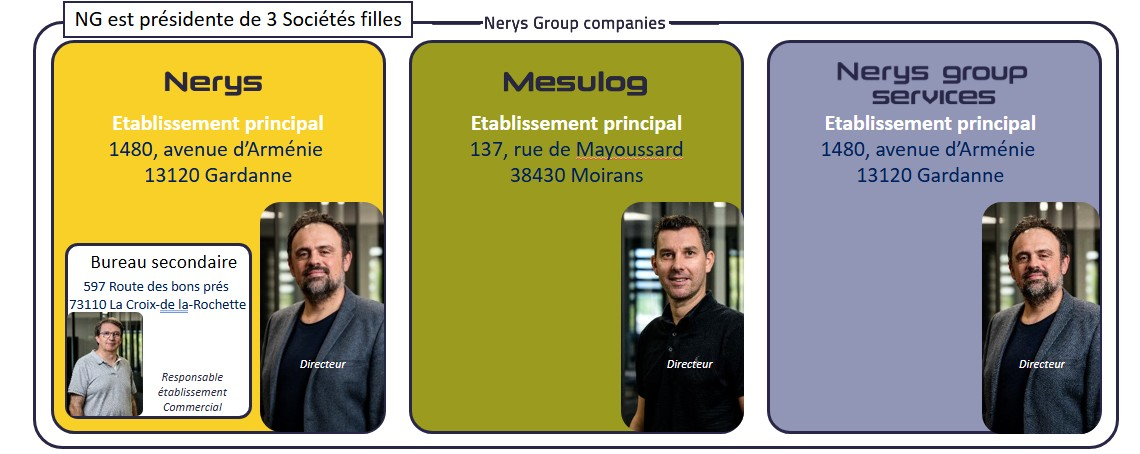
\includegraphics[width=0.7\textwidth]{images/sociétés.jpg}
    \caption{Présentation des sociétés filles de Nerys Group et de leurs directions}
    \label{fig:filiales-nerys}
\end{figure}
\par\bigskip


\subsubsection{Présentation du service d'accueil et de la hiérachie Mesulog}
\par\bigskip

\begin{figure}[h]
  \centering
  \begin{tikzpicture}[node distance=1.4cm and 1.6cm]

  \node[boxlight] (asaro) {Anthony Asaro\\Développeur technicien};
  \node[boxlight, left=1.8cm of asaro] (lerch) {Benjamin Lerch\\Développeur ingénieur};
  \node[boxlight, right=1.8cm of asaro] (bertin) {Thomas Bertin\\Développeur ingénieur};

  \node[boxlight, below=1.2cm of lerch] (sechi) {Kenzo Sechi\\Alternant};
  \node[boxlight, below=1.2cm of asaro] (kilian) {Verger Kilian\\Stagiaire};
  \node[boxgreen, below=1.2cm of bertin] (miquel) {Vianney Miquel\\Stagiaire};

  \node[boxmed, above=1.2cm of asaro, xshift=-3cm] (lamy) {Damien Lamy\\Chef de projet};
  \node[boxmed, above=1.2cm of asaro, xshift=3cm] (andrieu) {Adrien Andrieu\\Chef de projet};

  \node[boxdark, above=3.6cm of asaro] (president) {Luc Desruelle\\Directeur};

  \node[boxdark, right=2cm of president] (admin) {Emilie Evrard\\Responsable administrative};

  % --- Groupes par ligne (rectangle englobant) ---
  \node[draw=black, rounded corners=6pt, inner sep=8pt, fit=(president), label=north:{Direction}] (grp1) {};
  \node[draw=black, rounded corners=6pt, inner sep=8pt, fit=(lamy) (andrieu), label=above:{Chefs de projet}] (grp2) {};
  \node[draw=black, rounded corners=6pt, inner sep=8pt, fit=(lerch) (asaro) (bertin), label=above:{Développeurs}] (grp3) {};
  \node[draw=black, rounded corners=6pt, inner sep=8pt, fit=(sechi) (kilian) (miquel), label=above:{Stagiaires / Alternant}] (grp4) {};

  % --- Connexions entre rectangles seulement ---
  \draw[line] (grp1.south) -- ++(0,-0.6) -- (grp2.north);
  \draw[line] (grp2.south) -- ++(0,-0.6) -- (grp3.north);
  \draw[line] (grp3.south) -- ++(0,-0.6) -- (grp4.north);
  \draw[dashed] (admin.west) -- (grp1.east);

  \end{tikzpicture}
  \caption{Présentation de la hiérarchie de l'équipe Mesulog}
  \label{fig:hierachie-mesulog}
\end{figure}
\par\bigskip
Nous pouvons observer ci-dessus l'organigramme de l'équipe de Mesulog. L'équipe est composée de \textbf{Luc Desruelle}, qui est président de Nerys Group et assure le poste de directeur de Mesulog. Il est aussi le DSI de Mesulog.\\
Nous avons ensuite \textbf{Damien Lamy} et \textbf{Adrien Andrieu}, chefs de projet. Ils ont aussi des compétences de développeurs et présentent un profil technico-commercial. Le reste de l'équipe est composée de développeurs, à noter que Benjamin Lerch est également le RSSI du service informatique, il est donc mon surpérieur direct.\\
Nous avons ensuite \textbf{Kenzo Sechi}, alternant en informatique, qui travaille avec moi. Le stagiaire \textbf{Kilian Verger} est un stagiaire en BUT mesures physiques.\\
\textbf{Emilie Evrard} est quant à elle la responsable administrative de Nerys Group. Les activités de comptabilité et de ressources humaines étant mutualisées entre les entreprise du groupe. Certains acteurs exterieurs à l'équipe de Mesulog travaillent de concert avec l'équipe, notamment des salariés de Nerys et Nerys Groups Service. Cependant il ne sont pas représentés sur ce schéma organisationnel car je n'ai aucun contact avec eux dans mes mmissions.\\
\\
Je suis donc entouré d'une équipe expérimentée qui peut m'apporter de l'aide et des conseils en cas de problème. J'ai aussi un contact direct avec mes supérieurs que ce soit Benjamin Lerch ou Luc Desruelle, mon maitre de stage. Cela me permet de bénéficier d'un suivi régulier dans mes missions.
\newpage
\subsubsection{Présentation de l'environnement technique}
\begin{figure}[H]
\centering
\begin{adjustbox}{max width=0.98\textwidth,max totalheight=0.92\textheight}
\begin{tikzpicture}[
  node distance=1.0cm and 1.2cm,
  >=Stealth,
  font=\sffamily\tiny
]

%% ── ROW 0 : Internet ────────────────────────────────────────────────────────
\node[internet] (internet)
  {\textcolor{netblue}{\textbf{Internet}}};

%% ── ROW 1 : Routeurs (même hauteur, espacés) ────────────────────────────────
\node[dev=netblue, below left=1.6cm and 3.2cm of internet, text width=3.2cm] (adsl)
  {\textcolor{netblue}{\textbf{ADSL OVH Tel}}\\
   WAN: 109.190.53.59\\LAN: 192.168.10.1/24\\Ligne: 04 76 35 65 98};

\node[dev=netblue, below right=1.6cm and 3.2cm of internet, text width=3.2cm] (fibre)
  {\textcolor{netblue}{\textbf{Fibre Free Pro}}\\
   WAN: 45.80.27.81\\LAN: 192.168.10.0/24\\Ligne: 04 58 28 12 69};

%% ── ROW 2 : Firewall ────────────────────────────────────────────────────────
\node[dev=firered, below=3.2cm of internet, text width=3.8cm] (fw)
  {\textcolor{firered}{\textbf{Firewall Sophos XGS107}}\\
   WAN: 192.168.10.1/24\\LAN: 192.168.100.1/22\\
   P1:LAN · P2:WAN · P3:WiFi · P4:Codex};

%% ── ROW 3 : Switch Core ────────────────────────────────────────────────────

\node[dev=swgreen, below=2.0cm of fw, text width=3.2cm] (sw1)
  {\textcolor{swgreen}{\textbf{Switch Manageable}}\\
   Switch 1: 192.168.100.3\\
   VLAN Tel Ports 1–8};


\node[dev=swgreen, below=2.0cm of sw1, text width=3.2cm] (sw2)
  {\textcolor{swgreen}{\textbf{Switch Manageable}}\\
   Switch 2: 192.168.100.5\\
  };


%% ── VoIP ───────────────────────────────────────────────────────────────────

\node[dev=voiptel, left=4.8cm of sw1, text width=3.0cm] (voip)
  {\textcolor{voiptel}{\textbf{Téléphones VoIP}}\\
   Borne: 192.168.10.71\\
   04 58 00 16 71/72};

\node[dev=voiptel, below=0.2cm of voip, text width=3.0cm] (voip2)
  {\textcolor{voiptel}{\textbf{Téléphones VoIP}}\\
   Borne: 192.168.10.73\\
   04 58 00 16 71/74};


   \node[dev=voiptel, below=0.2cm of voip2, text width=3.0cm] (voip3)
  {\textcolor{voiptel}{\textbf{Téléphones VoIP}}\\
   Borne: 192.168.10.75\\
   04 58 00 16 71/76};


   \node[dev=voiptel, below=0.2cm of voip3, text width=3.0cm] (voip4)
  {\textcolor{voiptel}{\textbf{Téléphones VoIP}}\\
   Borne: 192.168.10.77\\
   04 58 00 16 71/78};

   \node[dev=voiptel, below=0.2cm of voip4, text width=3.0cm] (voip5)
  {\textcolor{voiptel}{\textbf{Téléphones VoIP}}\\
  Borne: 192.168.10.79\\
   04 58 00 16 71/78};



%% ── Switch Dev ─────────────────────────────────────────────────────────────

\node[dev=swgreen,
      right=3.5cm of sw2,
  text width=3.2cm,
  yshift=-50pt] (sw3) {
\textcolor{swgreen}{\textbf{Switch Manageable}}\\
Switch 3: 192.168.100.4
  };

%% ── Equipements Dev ────────────────────────────────────────────────────────



\node[dev=zonebg,
      above=5cm and of sw3,
      yshift=-50pt,
      text width=3.2cm] (unf)
{
\textcolor{wificolor}{\textbf{UNF Gateway}}\\
192.168.105.1
};


\node[dev=zonebg,
     right=0.5cm of unf,
      text width=3.2cm] (wifi)
{
\textcolor{wificolor}{\textbf{WiFi Ubiquiti}}\\
SSID: Mesulog\_Guest\\
192.168.106.1/24
};

\node[dev=devpurp,
      below right=1.0cm and 2cm of sw3,
      text width=3.2cm] (printer)
{
\textcolor{devpurp}{\textbf{HP LaserJet M254dw}}\\
192.168.101.110/22
};



%% ── ROW 6 (Devs) : PC Devs ─────────────────────────────────────────────────
\node[dev=devpurp, below=1cm of sw3, text width=3.5cm] (pcs)
  {\textcolor{devpurp}{\textbf{PC Developpeurs}}\\IP: 192.168.103.XXX/22};

%% ── ROW 4–6 (Serveurs) : sous le switch core ───────────────────────────────
%% Rangée A
\node[dev=srvoran, below left=4.2cm and 6.5cm of sw2, text width=3.4cm] (srv_vault)
  {\textcolor{srvoran}{\textbf{Serveur V4ULT}}\\
   Win Srv 2025\\IP: 192.168.100.111\\iLO: 192.168.100.112};

\node[dev=srvoran, right=0.4cm of srv_vault, text width=3.4cm] (srv_ad)
  {\textcolor{srvoran}{\textbf{Serveur AD}}\\
   Win Srv 2025\\IP: 192.168.100.113\\DNS + DHCP};

\node[dev=srvoran, right=0.4cm of srv_ad, text width=3.4cm] (srv_file)
  {\textcolor{srvoran}{\textbf{V4ULT-Files}}\\
   Win Srv 2025\\IP: 192.168.100.114\\S: / R: / T:};

%% Rangée B
\node[dev=srvoran, below=0.9cm of srv_vault, text width=3.4cm] (srv_bkp)
  {\textcolor{srvoran}{\textbf{Serveur Backup}}\\
   Win Srv 2025\\IP: 192.168.100.115\\Veeam Backup};

\node[dev=srvoran, right=0.4cm of srv_bkp, text width=3.4cm] (srv_waz)
  {\textcolor{srvoran}{\textbf{Serveur Wazuh}}\\
   Rocky Linux 10\\IP: 192.168.100.116\\Monitoring};

\node[dev=srvoran, right=0.4cm of srv_waz, text width=3.4cm] (nas)
  {\textcolor{srvoran}{\textbf{NAS2}}\\
   IP: 192.168.100.109/22\\Download NI};

%% Rangée C : Codex (pleine largeur, DMZ)
% Placé centré sous le serveur Wazuh
\node[dev=firered, below=0.8cm of srv_bkp, xshift=2cm, text width=7.4cm] (srv_cdx)
  {\textcolor{firered}{\textbf{Serveur Codex}}\\
   Rocky Linux 9\\
   LAN: 192.168.100.106~~WAN: 192.168.20.106\\
   Forge Tuleap};

\node[dev=srvoran, right=0.4cm of srv_cdx, text width=3.4cm] (suricata)
 {\textcolor{srvoran}{\textbf{Suricata}}\\
  Rocky Linux 10\\
  IP: 192.168.100.120/22\\
  Suricata et Evebox};

%% ════════════════════════════════════════════════════════════════════════════
%% ZONES DE FOND
%% ════════════════════════════════════════════════════════════════════════════
\begin{scope}[on background layer]
  \node[fit=(adsl)(fibre)(internet),
        rounded corners=8pt, fill=extbg, draw=netblue!30,
        dashed, line width=1pt, inner sep=10pt,
        label={[zonetitle=netblue]north west:Réseau Externe (WAN)}] {};

  \node[fit=(srv_vault)(srv_ad)(srv_file)(srv_bkp)(srv_waz)(nas)(srv_cdx),
        rounded corners=8pt, fill=servbg, draw=srvoran!40,
        dashed, line width=1pt, inner sep=10pt,
        label={[zonetitle=srvoran]above:Infrastructure Serveurs — 192.168.100.0/22}] {};

  \node[fit=(pcs)(sw3)(printer),
        rounded corners=8pt, fill=devbg, draw=devpurp!30,
        dashed, line width=1pt, inner sep=10pt,
        label={[zonetitle=devpurp]above:Zone Développeurs — 192.168.103.0/22}] {};

  \node[fit=(voip)(voip2)(voip3)(voip4)(voip5),
        rounded corners=8pt, fill=voipbg, draw=voiptel!40,
        dashed, line width=1pt, inner sep=8pt,
        label={[zonetitle=voiptel]above:VLAN -Téléphonie}] {};

  \node[fit=(unf)(wifi),
  rounded corners=8pt, fill=zonebg, draw=wificolor!40,
        dashed, line width=1pt, inner sep=10pt,
        label={[zonetitle=wificolor]above:Wifi invité — VLAN 192.168.105.0/24}] {};
\end{scope}

%% ════════════════════════════════════════════════════════════════════════════
%% CONNEXIONS
%% ════════════════════════════════════════════════════════════════════════════

%% Internet ↔ Routeurs
\draw[netbidi=netblue] (internet) -- (adsl);
\draw[netbidi=netblue] (internet) -- (fibre);

%% Routeurs → Firewall (arrivent sur les côtés du fw)
\draw[netlink=firered] (adsl.east)  -- ++(0.4,0) |- (fw.west);
\draw[netlink=firered] (fibre.west) -- ++(-0.4,0) |- (fw.east);

%% Firewall ↔ Switch Core
\draw[netbidi=swgreen, line width=1.6pt]
  (fw.south) -- node[right, font=\sffamily\tiny, text=swgreen]{192.168.100.1/22}
  (sw1.north);


%%sw1 -> sw2
\draw[netbidi=swgreen, line width=1.6pt]
  (sw1.south) -- node[right, font=\sffamily\tiny, text=swgreen]{
    192.168.100.1/22
  }
  (sw2.north);


%% Switch Core ↔ Switch 3
\draw[netbidi=devpurp] (sw2.east)  -- ++(0.4,0) |- (sw3.west);

%% Switch Core ↔ VoIP
\draw[netbidi=voiptel] (sw1.west) -- (voip.east);

\draw[netbidi=devpurp, line width=1.2pt] (sw3) -- (pcs);


%% Switch Core ↔ Serveurs (lien central vers srv_ad)
\draw[netbidi=srvoran, line width=1.6pt]
  (sw2.south) -- ++(0,-0.55) -| (srv_ad.north);

\draw[netbidi=netblue] (unf) -- (wifi);
% Lien Firewall ↔ UNF avec double coude bleu
\draw[netbidi=netblue, line width=1.2pt] (fw.east)  -- ++(0.4,0) |- (unf.west);

\draw[netbidi=devpurp]  (sw3.east)  -- ++(3.4,0) -|(printer.north);


%% Firewall → Codex (Port 4 WAN, tirets)
\draw[netlink=firered, dashed, line width=1.2pt]
  (fw.south) -- ++(0,-0.3) -- ++(-12.8,0) |- (srv_cdx.west);

%% ════════════════════════════════════════════════════════════════════════════
%% LÉGENDE + TITRE
%% ════════════════════════════════════════════════════════════════════════════
\node[anchor=south east, font=\sffamily\tiny, align=right, text width=8cm]
  at (current bounding box.south east) {
  \textcolor{swgreen}{—\,LAN interne}~~
  \textcolor{devpurp}{—\,ZoneDevs}~~
  \textcolor{srvoran}{—\,Zone Serveurs}~~
  \textcolor{firered}{--\,WAN/DMZ (trait plein : liaison directe ~/~ pointillé : liaison via reverse proxy exposée sur Internet)}~~
  \textcolor{voiptel}{—\,VoIP}
};

\end{tikzpicture}
\end{adjustbox}
\caption{Plan réseau de Mesulog en 2026}
\label{fig:plan-reseau}
\end{figure}
\par\bigskip

Voici l'architecture réseau de Mesulog. Le réseau comporte un VLAN pour la téléphonie, un LAN physique pour le wifi et des zones d'adressages, une pour les serveurs et une pour les ordinateurs des employés. Il n'y a donc pas de segmentation réseau réelle entre la zone serveur et la zone employés.
Nos serveurs sont hébergés sur un hyperviseur Hyper-V, Serveur V4ULT, à l'exception du serveur Suricata et du NAS.\\
Les serveurs de l'infrastructure sont regroupés sous le nom de domaine interne \textbf{V4ULT}, on y retrouve notamment :
\par\bigskip
 \begin{itemize}
  \item[$\bullet$] \textbf{V4ULT-AD} : l'Active Directory (Serveur \href{https://fr.wikipedia.org/wiki/LDAP}{LDAP}) faisant aussi office de Serveur DHCP et DNS.
  \item[$\bullet$] \textbf{V4ULT-FILES} : Le seveur de de fichiers de l'entreprise découpés en 3 entités (Echanges, Mesulog, Downloads)
  \item[$\bullet$] \textbf{Server Backup} : Le serveur de sauvegarde de l'entreprise utilisant Veeam Backup \& Replication.
  \item[$\bullet$] \textbf{Server Codex} : Instance de Tuleap, similaire à GitLab, gestionnaire de version de code source basé SVN. Le serveur est exposé sur internet derrière un reverse proxy et un firewall.
 \end{itemize}
\par\bigskip
Quant à l'environnement logiciel, les utilisateurs, principalement des développeurs NI LabVIEW \& NI TestStand, utilisent Windows 11 avec la suite de logiciels suivante :
\par\bigskip

\begin{itemize}
  \item[$\bullet$] \textbf{\href{https://www.virtualbox.org/}{Oracle VirtualBox}} : virtualisation pour exécuter des machines virtuelles locales.
  \item[$\bullet$] \textbf{\href{https://www.microsoft.com/fr-fr/microsoft-365/}{Suite Microsoft 365}} : bureautique et collaboration (Outlook, Word, Excel, Teams...).
  \item[$\bullet$] \textbf{\href{https://www.mozilla.org/fr/firefox/}{Firefox}} : navigateur web principal pour la navigation et les outils web internes.
  \item[$\bullet$] \textbf{\href{https://www.teamviewer.com/}{TeamViewer}} : assistance à distance et support technique.
\end{itemize}
\par\bigskip

Les logiciels utilisés dans les machines virtuelles peuvent être les suivants :
\par\bigskip

\begin{itemize}
  \item[$\bullet$] \textbf{NI LabVIEW} : environnement de développement pour les applications de test et mesure.
  \item[$\bullet$] \textbf{NI TestStand} : Séquenceur de tests automatisés.
  \item[$\bullet$] \textbf{Logiciels propriétaires clients} : applications spécifiques fournies par des clients (e.g. ?)
\end{itemize}

\subsection{Objectifs et organisation des missions}
\par\bigskip
Durant mon stage, J'ai pu effectuer plusieurs missions, certaines étaient prévues à l'avance, d'autres sont apparues au fur et à mesure de l'avancement du stage.
L'objectif initial de ce stage était la mise en place d'outils de supervision et de management d'évenements de sécurité, tels que Suricata et Wazuh.\\
Cependant ce n'est pas la première mission que j'ai effectuée, en effet pour aprehender ce nouvel environnement j'ai commencé par une mission d'analyse et de mise en forme de données sur une base de données Access.\\
J'ai ensuite mis en place Suricata, un IDS open source, afin de surveiller les évenements réseau. Suite à quoi j'ai installé et configuré le SIEM open-source Wazuh.\\
J'ai aussi pu retravailler l'organisation de l'Active Directory de l'entreprise, avec des mises en place de GPO, ou encore participé à la création d'un campagne interne de test de phishing. Certaines plus petites tâches se sont intercalées entre ces sujets principaux, elle ne seront pas détaillées dans ce rapport.\\
\\
Ces missions étant toutes étroitement liées entre elles, excepté l'analyse de données pour un client, elles se sont déroulées en parallèles sur la durée de mon stage.
par\bigskip
\begin{figure}[H]
\centering
\resizebox{\textwidth}{!}{%
  \begin{ganttchart}[
      hgrid style/.style={draw=gray!20, line width=0.4pt},
      vgrid={*{6}{draw=none}, dotted},
      time slot format=isodate,
      time slot unit=day,
      canvas/.style={draw=gray!30, line width=0.5pt},
      title/.style={draw=none, fill=gray!12},
      title label font=\small\bfseries\color{black!70},
      title height=1,
      bar label font=\small,
      bar label node/.append style={align=right, text width=6cm},
      bar height=0.55,
      bar top shift=0.225,
      y unit title=0.7cm,
      y unit chart=1.2cm,
      x unit=0.16cm
    ]{2026-04-13}{2026-07-17}
      \gantttitlecalendar{year, month=name} \\
      \ganttbar[bar/.append style={fill=teal!30, draw=teal!50, rounded corners=2pt}]
          {Analyse de données client dans Microsoft Access}{2026-04-13}{2026-05-03} \\
      \ganttbar[bar/.append style={fill=blue!30, draw=blue!50, rounded corners=2pt}]
          {Installation de Suricata et Evebox}{2026-05-04}{2026-06-07} \\
      \ganttbar[bar/.append style={fill=teal!30, draw=teal!50, rounded corners=2pt}]
          {Installation et Configuration de Wazuh}{2026-05-11}{2026-06-28} \\
      \ganttbar[bar/.append style={fill=blue!30, draw=blue!50, rounded corners=2pt}]
          {Durcissement système (GPO) et refonte de l'organisation Active Directory}{2026-05-31}{2026-07-17} \\
      \ganttbar[bar/.append style={fill=teal!30, draw=teal!50, rounded corners=2pt}]
          {Réalisation d'une campagne de phishing}{2026-06-15}{2026-07-05} \\

  \end{ganttchart}
}%
\caption{Chronologie des missions réalisées pendant mon stage}
\label{fig:gantt-missions}
\end{figure}
\section{Réalisation}

\subsection{Base de données Access}

  Au début de mon stage, j'ai travaillé sur une analyse de base de donnée Microsoft Access pour un client de Mesulog. Cette base de donnée, générée automatiquement depuis les rapports de test de banc de test Mesulog présent chez des clients, ce présente au départ comme 1 seule table à 23 colonnes.\\
  \begin{figure}[H]
    \centering
    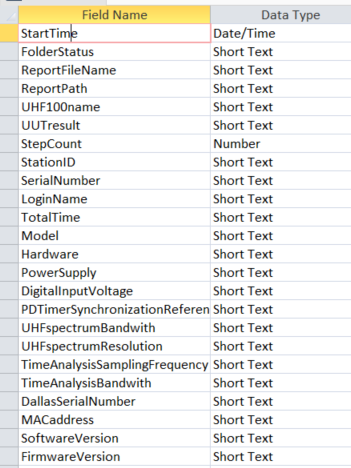
\includegraphics[width=0.6\textwidth]{images/access-schema.png}
    \label{fig:access-sechema}
    \caption{Schéma de la table initiale}
  \end{figure}
  \par\bigskip
  Il était donc courant d'avoir des enregistrements partiels, erronés ou avec un mauvais format. L'objectif final était de produire différents graphiques et tableaux pour analyser l'évolution de la production de modules, appelés "V1" ou "V2".\\
  \\
  Les modules sont testés sur un banc, ils sont soit de type 1 ou 2. Un module passe un ou plusieurs tests ou essais avant d'être validé. Pour qu'un module soit validé il suffit d'un essai passé. Un essai à 4 issues : "Passed" (valide), "Failed" (non-valide), "Terminated" (le test s'est treminé prématurément) et "Error" (le banc de test a fait crasher le test).\\
  \\
  Nous devons donc produire un tableau récapitulatif général par année et par banc avec entre autre les nombres de modules validés, le nombre d'essais moyen et médian avant pour un moduel avant d'être validé, le temps moyen en heure pour valider un module, le ratio des états des essais.\\
  \\
  Le client a aussi 2 demandes plus particulières : \\
  \begin{enumerate}
    \item[$\bullet$] Nous devons analyser plus précisément les états des essais les lundi matins car un nombre anormal d'erreurs sur le banc est suspecté.
    \item[$\bullet$] Nous devons aussi analyser la distribution des états des essais selon le pas de test. En effet une séquence d'essais complète comporte 39 étapes.
  \end{enumerate}
\par\bigskip

\subsubsection{Nettoyage des données}

  Pour pouvoir correctement exploiter les données, il est important d'avoir des données complètes et sous le même format.\\
  Les colonnes comportant des erreurs ou des oublis sont principalement :\\
  \begin{enumerate}
    \item[$\bullet$] Le numéro de série du module, qui comporte parfois des espaces, lettres minuscule ou un mauvais nombre de caractères.
    \item[$\bullet$] Le type du module (V1 ou V2), qui est noté UHF100 pour V1, UHF100 V2 ou UHF1002Ghz. Cette valeur est souvent manquante, il faut donc l'inférer.
    \item[$\bullet$] Les essais qui font partis de la chaine production et les essais de R\&D ou de SAV qui ne sont pas signalés de manière consistante. Il faut écarter ces enregistrements de l'analyse.
  \end{enumerate}
\par\bigskip
  Pour ce faire nous avons créé une suite de requètes SQL pour automatiquement effecture ce nettoyage. Etant donné que l'objectif final est d'automatiser l'execution de toutes ces requètes dans Microsoft Access avec un scipt VBS (Visual Basic Scripting), la synthaxe SQL utilisée est celle de Microsoft Access, qui nous impose des choix parfois sous-optimaux.\\
  Pour ne pas surcharger ce rapport nous verrons ici seulement un exemple de formattage, le reste est disponible en \hyperref[fig:setup-access]{Annexe} :
  \par\bigskip
  \begin{figure}[H]
    \lstinputlisting[language=SQL, firstline=122, lastline=141]{Annexe/Setup_query.sql}
    \label{fig:setup-access-08}
    \caption{Requête de normalisation des fins de numéro de série}
  \end{figure}
\par\bigskip

Nous pouvons voir ci-dessus un requête destinée à formatter tous les numéros de série sous la forme "*.XXX", "XXX" étant 3 chiffres.\\
Exemple : "17A240923.2" est transformé en "17A240923.002"\\
Afin de ne perdre aucune information, le numéro de série normalisé est inséré dans une nouvelle colonne. Il en va de même pour le modèle et pour l'objectif du test (Porduction ou SAV, R\&D).\\
\\
Une fois que toutes les données sont complétées et formattées, nous passons à l'exploitation de celles-ci.
\par\bigskip
\subsubsection{Extraction des données pertinentes}

L'objectif de cette partie est de remplir un tableau type comme présenté ci-dessous :\\
\begin{figure}[H]
    \centering
    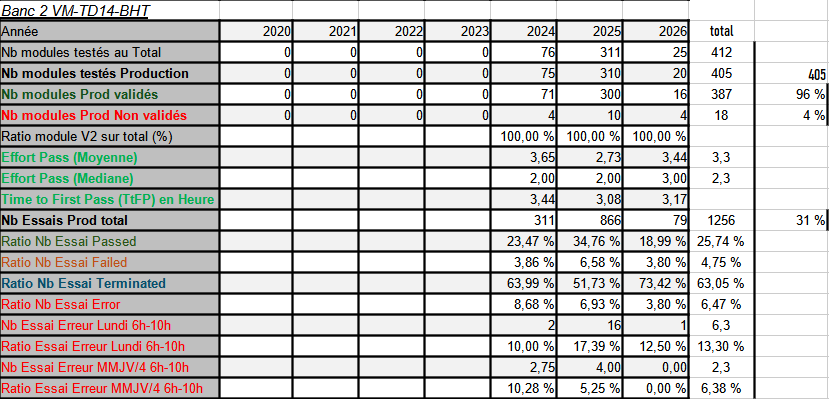
\includegraphics[width=1\textwidth]{images/tableau-access.png}
  \label{fig:tableau}
  \caption{Tableu récapitulatif général - (pour le banc VM-TD14-BHT)}
\end{figure}

Ce tableau récapitulatif permet de voir facilement l'évolution de l'utilisatiion du banc, des résultats d'essais et du nombre de modules sortis en production.\\
Pour plus de précision, le "Effort to Pass" est le nombre d'essais avant une réussite, tandis que le "Time to First Pass" est  le temps cumulé de tous les essais jusqu'à un essais validant.\\
Nous pouvons aussi voir des lignes mettant en évidence les différences d'essais en erreur entre les lundis matins et les autres jours de la semaine.\\
\\
Dans ce jeu de données, nous avons 2 bancs est 2 types de modules. Il était demandé d'analyser l'évolution de la production par banc tous types de modules confondus et par banc seulement pour les modules types V2. Cela nous fait donc 6 tableaux à remplir de données.\\
Pour extraire ces données, nous partons de la table nettoyée, et nous avons fait une suite de 18 requêtes SQL pour extraire les données ou créer des tables temporaires pour d'autres requêtes. Si dans ces requêtes nous définissons le banc et le type de module en dur, il est prévu d'utiliser un script VBS (Visual Basic Scripting) pour remplacer automatiquement ces variables dans les reqêtes.
\newpage
Comme précedement, nous ne montrons pas l'intégralité des requêtes dans le corps du rapport, mais elles sont disponibles en \hyperref[fig:extraction-access]{ici}.
\begin{figure}[H]
  \lstinputlisting[language=SQL, firstline=411, lastline=448]{Annexe/BANC_MOD_extraction_query.sql}
  \label{fig:extraction-access-15}
  \caption{Requête d'une table tamporaire pour le calcul du TtFP (Time to First Pass)}
\end{figure}
\par\bigskip
Cette requête créer une table temporaire qui regroupe l'empreinte temporelle du premier essai d'un module, du premier essai validant, de la différence entre ces deux essais, du temp d'essai du second essai et finalement du "Time to First Pass" arrondi à l'heure.
\newpage
Maintenant que nous avons extrait toutes les données nécessaires, nous pouvons les mettre en forme, voici donc quelques exemples de graphiques produits (L'ensemble est trouvable en \hyperref[fig:graphiques]{Annexe}):
\begin{figure}[H]
    \centering
    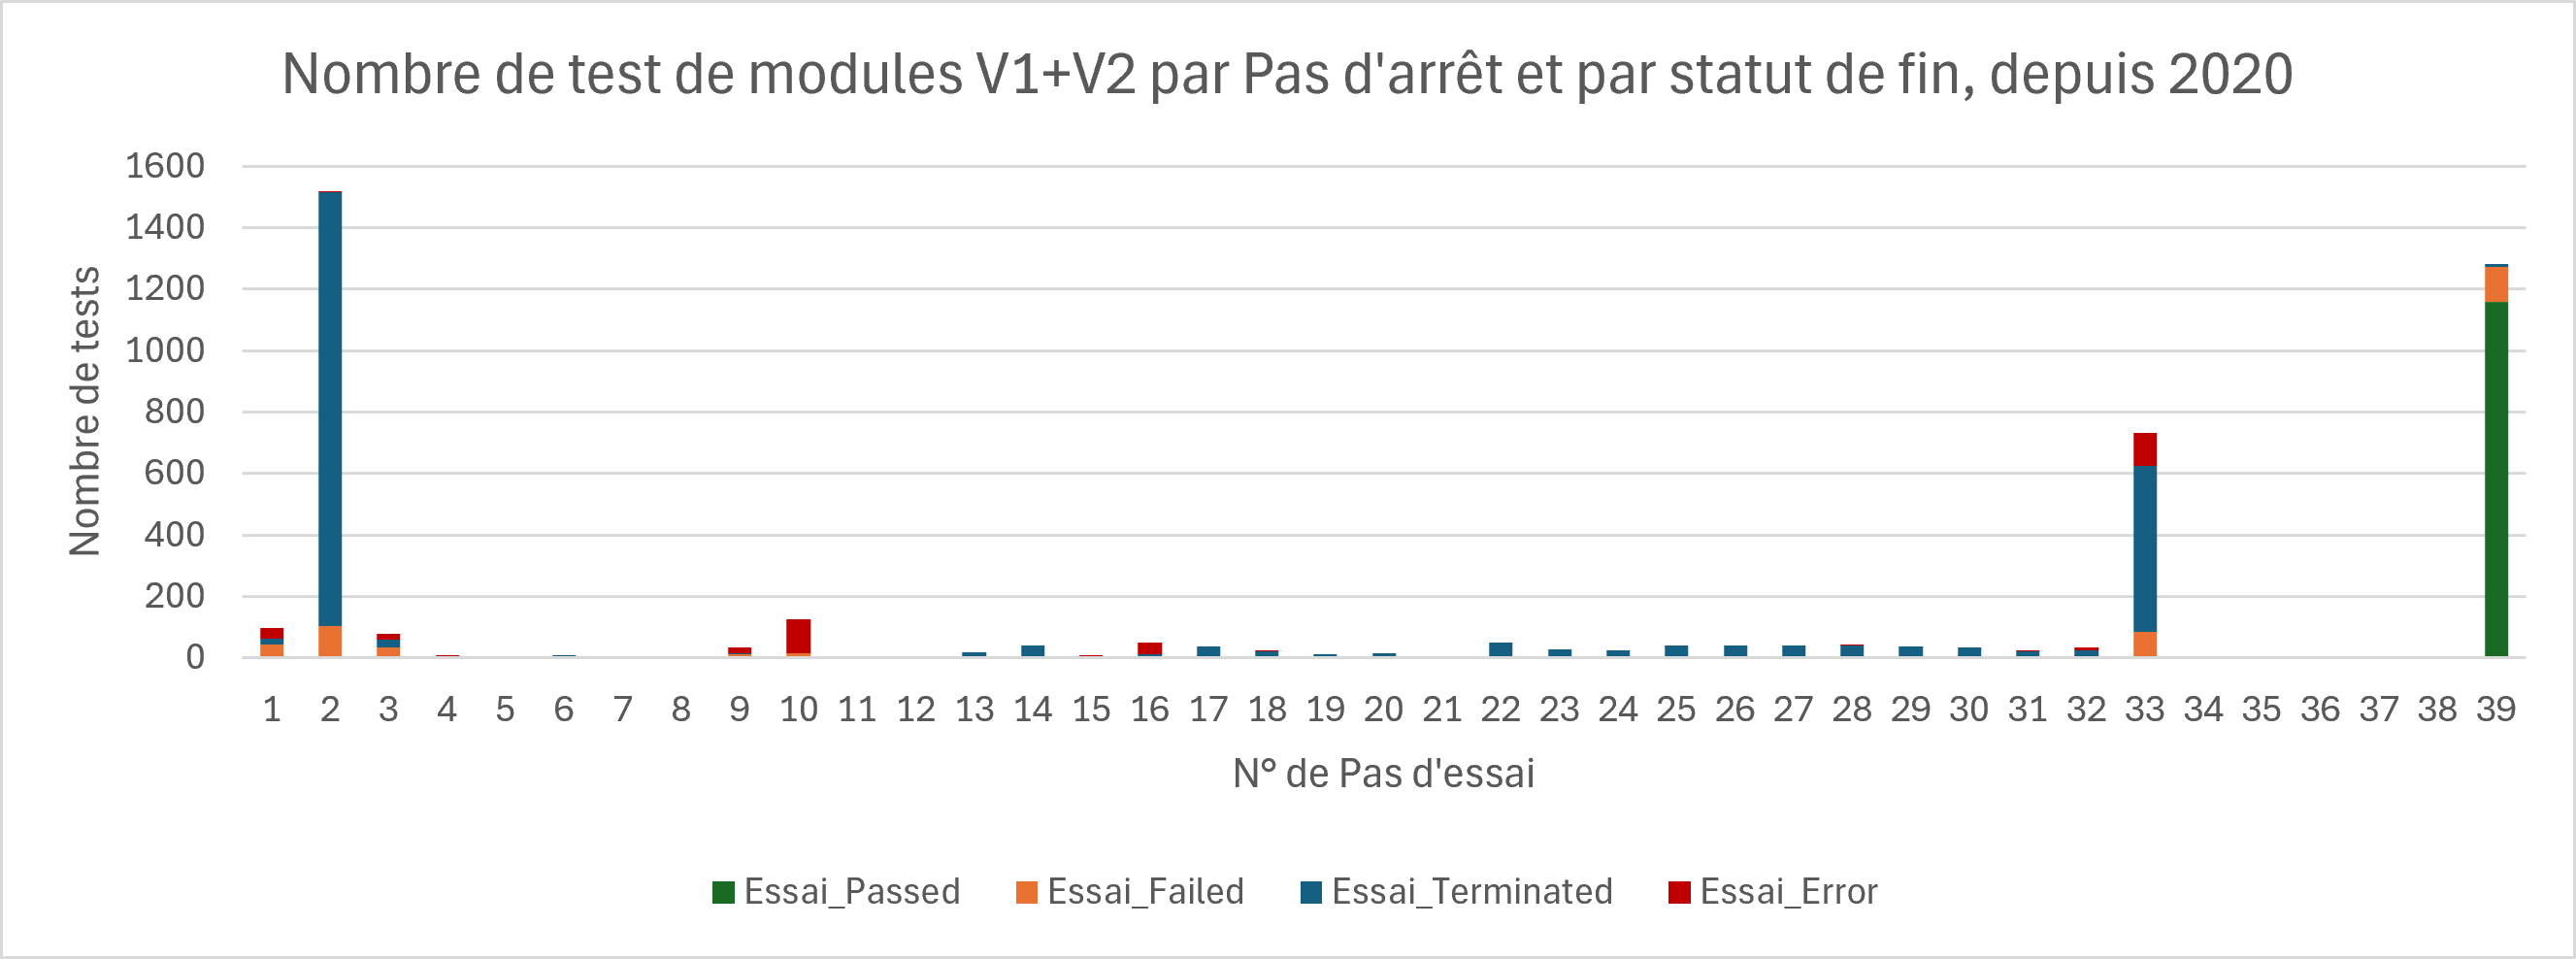
\includegraphics[width=1\textwidth]{images/nb_test_mod12_stepcount.png}
  \label{fig:graph-step12-corps}
  \caption{Distribution des statuts de fin des essais par étape de l'essai, tous bancs confondus}
\end{figure}
\par\bigskip
\subsection{Mise en place de Suricata}

Suricata est un système de détection/prévention d'intrusion. Son fonctionnement est assez simple : il capture chaque paquet qui transite sur le réseau et analyse ses propriétés.Pour engendrer une alerte ou une action, Suricata utilise des règles, qui sont un ensemble de paramètres. Si une trame correspond à tous les critères (elle à la même signature) alors une action est prise par suricata.
\begin{figure}[H]
    \centering
    \lstinputlisting[language=bash]{Annexe/suricata-example.rules}
  \label{fig:example-rule-corps}
  \caption{Exemple de règle Suricata - ici une règle contre le mDNS poisoning}
\end{figure}
Suricata peut donc décider de ne rien faire, de génerer une alerte ou de rejetter la trame en mode IPS (Intrusion Prevention System). En mode IDS (Intrusion Detection System) nous lancons simplement des alerts mais sans bloquer le traffic. C'est comme ça que nous l'installerons, afin d'éviter qu'un faut positif coupe une connexion légitime.\\
 Pour installer Suricata, nous avons pris une machine physique.   Pour éviter de risquer ralentir le traffic, nous avons mis en place un port mirroring à partir d'un swirch juste en aval du pare-feu Sophos, le suricata reçoit donc une copie exacte de tout le traffic qui passe de WAN à LAN et de LAN à WAN.\\
 \\
 La distribution linux utilisée en production à mesulog est Rocky Linux 10, une distribution RHEL (Red Hat).   L'installation de suricata sur Rocky Linux se fait avec le dépôt COPR du projet OISF (développeurs et mainteneurs de Suricata).
 \newpage
  Cependant ce dépôt qui installe via un fichier rpm n'arrive pas à résoudre ses dépendance sur Rocky 10. Nous avons donc choisit d'installer suricata via l'image docker fournie par Jason Ish, membre du projet OISF.\\
  Ce choix technique nous permet aussi d'installer Evebox dans un second conteneur docker. Evebox est l'outil de gestion d'alerte et d'évenement pour Suricata développé et maintenu lui aussi par le projet OISF.
  Ces 2 conteneurs sont réunis dans un même fichier docker compose pour une meilleure maintenabilité.
\begin{figure}[H]
    \centering
    \lstinputlisting[basicstyle=\small]{Annexe/compose.yaml}
  \label{fig:compose-yaml}
  \caption{fichier Docker Compose}
\end{figure}
\par\bigskip
Premièrement nous pouvons voir que les deux conteneurs sont paraméter pour redémarrer automatiquement dès qu'ils sont éteints, pour limiter le temps hors-service. La variable d'environnement "TZ" permet de s'assurer que l'heure soit bien synchronisée dans les logs.\\
Quelques points important :\\
  \begin{enumerate}
    \item[$\bullet$] Des capabilités ont été ajoutées avec "cap\_add" au conteneur Suricata pour accéder à l'interface réseau de la machine hôte, créer des sockets ou changer la priorité des processus si besoin.
    \item[$\bullet$] La variable d'environnement "EVEBOX\_RETENTION\_PERIOD" permet de définir un limite de temps au delà de laquelle les logs sont effacés, très important pour ne pas saturer le stockage. Ici la limite est de 7 jours.
  \end{enumerate}
  \par\bigskip

Ci-dessous l'interface web de Evebox, qui permet de suivre pas seulement les alertes mais tous les évenemment Suricata : \\
\begin{figure}[H]
    \centering
    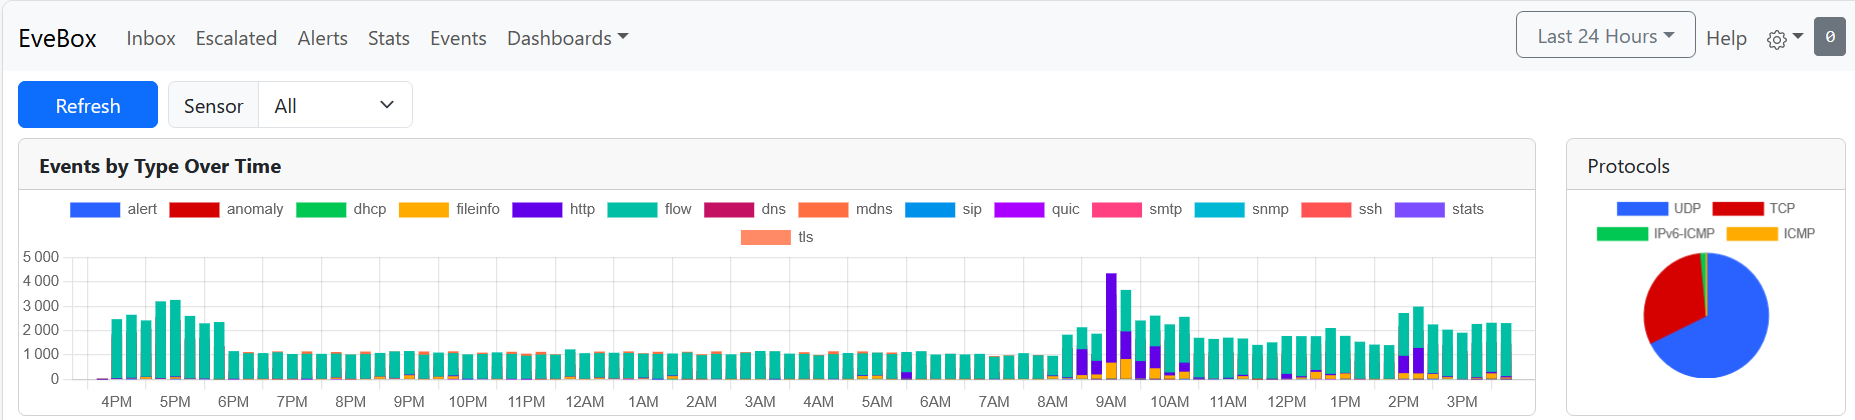
\includegraphics[width=1\textwidth]{images/evebox-interface.png}
  \label{fig:evebox-interface}
  \caption{Interface web d'Evebox}
\end{figure}
\newpage
\subsubsection{Configuration et integration avec Wazuh}

Pour éviter de surcharger le SIEM, nous avons créé un deuxième fichier de log sous le format EVE (Extensible Event Format), intitulé eve-wazuh.json, dans lequel seulement les alertes Suricata sont loggées, contrairement au fichier de log eve.json pour Evebox où toutes les alertes ainsi que tous les évenement sont loggés.\\
Ainsi nous avons un agent wazuh sur la machine hôte Rocky linux de suricata et evebox. Cet agent est configuré pour utiliser le fichier eve-wazuh.json comme source.\\
Cet agent wazuh a aussi une deuxième fonction ; en effet il vérifie régulièrement l'état des conteneurs dockers, et remonte des alertes dans wazuh dès qu'un changement d'état ou une commande docker est lancée sur la machine.\\
Il suffit par la suite de créer des règles dans Wazuh pour attraper les alertes suricata pertinentes.\\
\par\bigskip
\begin{figure}[H]
    \centering
    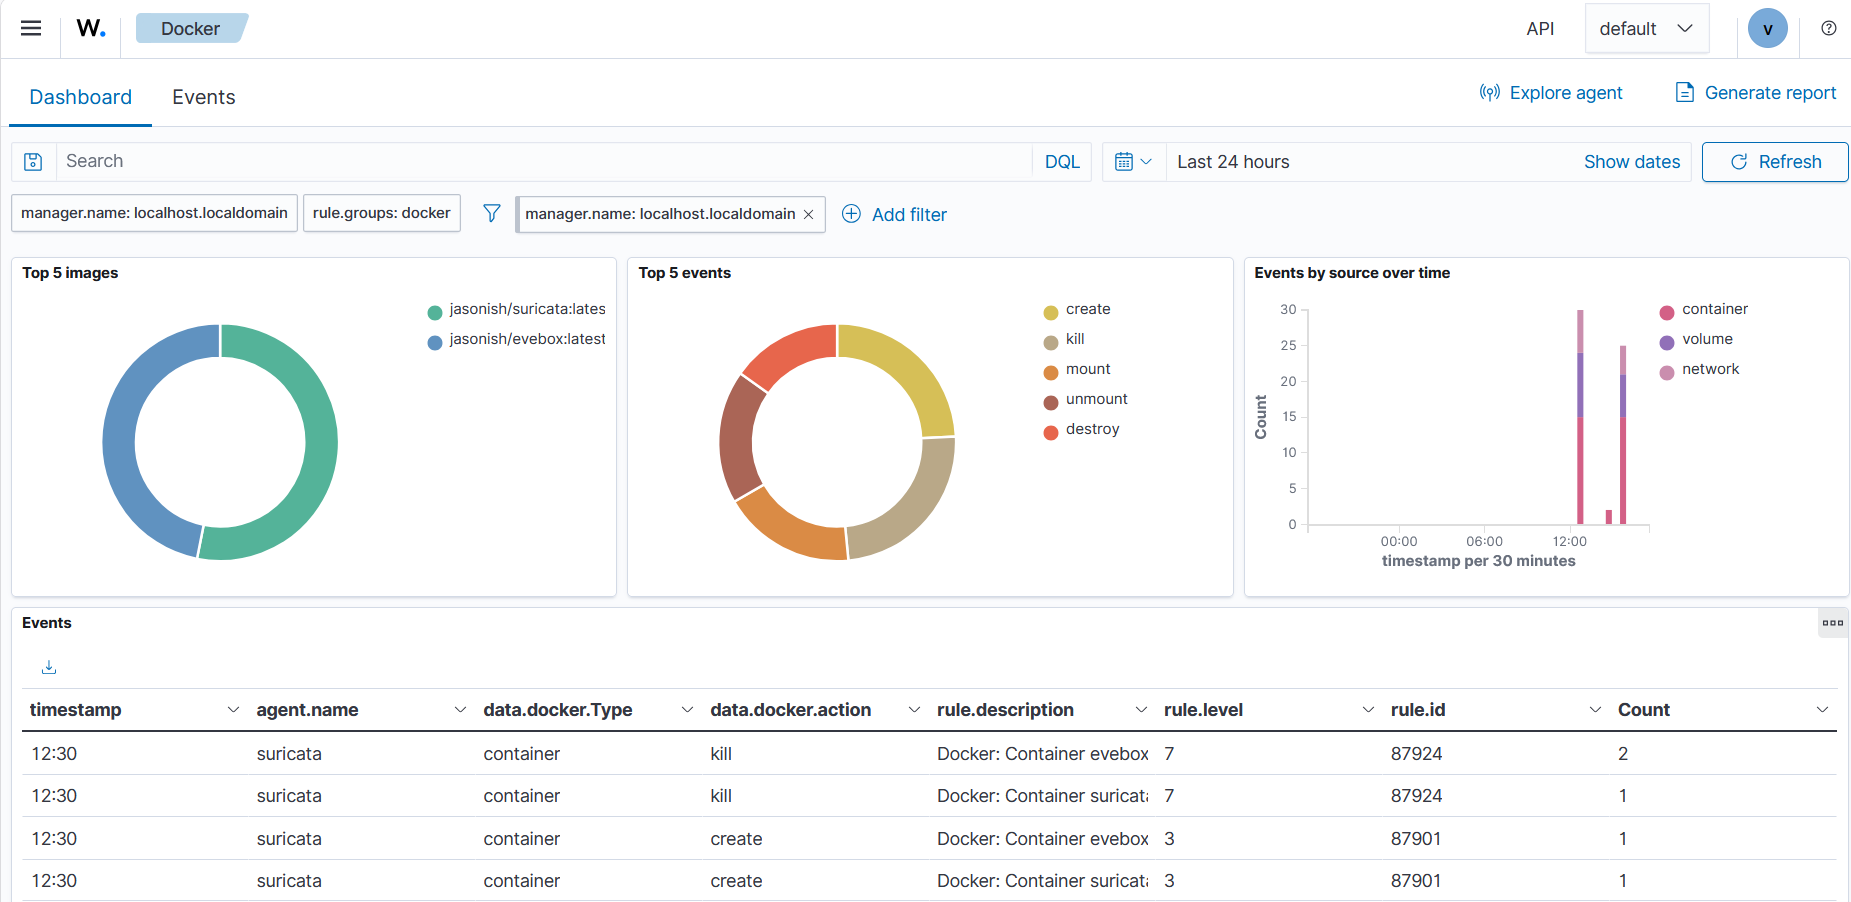
\includegraphics[width=1\textwidth]{images/docker-wazuh.png}
  \label{fig:docker-wazuh}
  \caption{Dashboard d'évenement Docker dans Wazuh}
\end{figure}
\par\bigskip
En ce qui concerne les règles de Suricata en mode IDS, nous avons premièrement ajouté les règles de l'Open Emerging Threats publiées par Proofpoint. Avec des règles additionnnelles, ajoutées à la suite de l'analyse de l'activité réseau avec Evebox.\\
Par exemple, en constatant un traffic significatif de packets mDNS sur le réseau, des règles contre le mDNS poisoning on été ajoutées dans un fichier de règle supplémentaire.\\
Afin de se prémunir contre les IPs malicieuses, nous avons ajouté des règles automatiquent suivant une liste d'ip malicuese.\\
Pour ce faire, nous avons écrit un programme bash qui récupère des listes d'ip maliceuses depuis de listes de emerging threats, abuse.ch ou encore alien vault (Voir annexe). Nous concatenons ensuite ces liste dans un seul fichier, puis ajountons pour chaque ip 2 règles dans un fichier de règle suricata "ip-reputation.rules"
une règle pour les connexions sortante et la deuxième pour les connexions entrantes depuis/vers cette ip. Ensuite le programme execute "docker kill --signal=USR2 suricata" qui envoie un signal non pas d'arrêt mais de reload des règles à chaud sans redémarrer le service.\\
Ce reload est d'ailleurs détecté par l'agent wazuh présent sur la machine hôte, qui remonte un évenement de reload dans wazuh.\\
\newpage
\begin{figure}[H]
    \centering
    \lstinputlisting[language=bash, basicstyle=\tiny]{Annexe/suricata-ip-update.sh}
  \label{fig:suricata-ip-update}
  \caption{Programme de mise à jour automatique des règles d'ip malicieuses}
\end{figure}
\par\bigskip
Pour executer ce programme de manière automatique, nous avons créé un service linux "suricata-ip-update.service" qui est lancé tous les jours à minuit par "suricata-ip-update.timer".\\
Grâce à l'option "RandomizedDelaySec=1800", ce timer a une fenêtre de 30 min (entre 00:00 et 00:30) pour lancer le service, ce qui permet d'éviter de surcharger la machine si des processus louds sont déjà en train de s'executer (backup automatiques entre autre).\\
\newpage
\begin{figure}[H]
    \centering
    \lstinputlisting[]{Annexe/suricata-ip-update.timer}
  \label{fig:suricata-ip-update-timer}
  \caption{Timer pour le service linux suricata-ip-update}
\end{figure}
\par\bigskip
\begin{figure}[H]
    \centering
    \lstinputlisting[]{Annexe/suricata-ip-update.service}
  \label{fig:suricata-ip-update-service}
  \caption{Serice linux suricata-ip-update}
\end{figure}
\par\bigskip

\subsection{Installation et Intégration de Wazuh}

En parallèle de l'installation de suricata, nous avons mis en place un SIEM (Outil de gestion d'évenement et d'informations de securité). Nous avons opté pour le SIEM Open source Wazuh.\\
En effet, il est important pour une entreprise qui manipule des données client parfois très confidentielles de superviser et surveiller le réseau pour détecter toute panne, attaque ou utilisation inappropriée des ressources.
Un SIEM marche donc main dans la main avec des systèmes IDS pour garantir une meilleure sécurité du système d'information. Le SIEM sert aussi de centralisateur et archiveur de logs, ce qui permet de remplir des critères ISO 270001.\\
Wazuh est installé sur une machine Rocky Linux 10 dans une VM contrairement à suricata qui est une machine physique.
\newpage
\subsubsection{Présentation de Wazuh et de son fonctionnement}
Wazuh est un SIEM (Security Information and Event Management), c'est un outil qui permet de regrouper tous les évenements réseau et les analyser pour ensuite détecter une menace ou un disfonctionnement.\\
Pour récuperer tous ces journaux, Wazuh marche de concert avec des agents, installés sous forme de services d'arrière-plan. Ces agents récupèrent les logs de l'appareil et les transmettent au serveur Wazuh. Dans le cas où il est impossible d'installer un agent Wazuh sur l'appareil à monitorer, il est possible d'envoyer directement les journaux vers le serveur Wazuh sur une connexion UDP ou TCP, à condition de définir dans la configuration de Wazuh le format des logs et le port d'écoute.\\
\\
\begin{figure}[H]
  \begin{center}
  \begin{tikzpicture}[
    >=Stealth,
    % Style boîte grise standard
    greybox/.style={
      draw=greyborder, fill=greybox,
      rounded corners=4pt,
      align=center,
      font=\small,
      minimum width=3.2cm,
      minimum height=1.1cm,
      inner sep=6pt
    },
    % Style boîte bleue (Manager / Indexer)
    bluebox/.style={
      draw=blueborder, fill=bluelight,
      rounded corners=6pt,
      align=center,
      font=\small,
      inner sep=8pt
    },
    % Style boîte interne du manager
    innerbox/.style={
      draw=greyborder, fill=greybox,
      rounded corners=3pt,
      align=center,
      font=\small,
      minimum width=2.8cm,
      minimum height=1.0cm,
      inner sep=5pt
    },
    % Flèches
    arrow/.style={->, thick, color=gray!70},
    % Label de flèche
    arrowlabel/.style={font=\footnotesize, color=gray!80, midway}
  ]

  %% ============================================================
  %% RANGÉE 1 : Endpoints surveillés (cadre pointillé)
  %% ============================================================

  % Agent Linux
  \node[greybox] (linux) at (-4, 0) {
    \textbf{Agent Linux}\\[2pt]
    \footnotesize Collecte logs,\\syscalls, fichiers
  };

  % Agent Windows
  \node[greybox] (windows) at (0, 0) {
    \textbf{Agent Windows}\\[2pt]
    \footnotesize Collecte logs,\\registre, audits
  };

  % Agent Cloud
  \node[greybox] (cloud) at (4, 0) {
    \textbf{Agent Cloud}\\[2pt]
    \footnotesize AWS, Azure,\\GCP, Docker
  };

  % Cadre pointillé "Endpoints surveillés"
  \begin{scope}[on background layer]
    \node[draw=dashedborder, dashed, rounded corners=8pt,
          fit=(linux)(windows)(cloud),
          inner sep=14pt,
          label={[font=\small, color=dashedborder]above left:Endpoints surveillés}
        ] (endpoints) {};
  \end{scope}

  %% ============================================================
  %% LABEL TLS
  %% ============================================================
  \node[font=\footnotesize, color=gray] (tls) at (-3, -1.2) {Chiffré (TLS)};

  %% ============================================================
  %% RANGÉE 2 : Wazuh Manager (boîte bleue avec composants internes)
  %% ============================================================

  % Composants internes du Manager
  \node[innerbox] (rules) at (-2.2, -4.2) {
    \textbf{Rules Motor}\\[1pt]
    \footnotesize 3000+ règles intégrées
  };

  \node[innerbox] (decoders) at (2.2, -4.2) {
    \textbf{Decoders}\\[1pt]
    \footnotesize Parsing des logs
  };

  \node[innerbox] (fim) at (-3.2, -5.8) {
    \textbf{FIM}\\[1pt]
    \footnotesize Intégrité
  };

  \node[innerbox] (sca) at (0, -5.8) {
    \textbf{SCA}\\[1pt]
    \footnotesize Conformité
  };

  \node[innerbox] (vuln) at (3.2, -5.8) {
    \textbf{Vuln.}\\[1pt]
    \footnotesize CVE
  };

  % Titre du Manager (au-dessus des composants)
  \node[font=\normalsize\bfseries, color=black] (managertitle) at (0, -3.0) {Wazuh Manager};
  \node[font=\small, color=bluetext] (managersubtitle) at (0, -3.45)
        {Cœur du système — analyse et corrélation};

  % Cadre bleu du Manager
  \begin{scope}[on background layer]
    \node[bluebox,
          fit=(managertitle)(managersubtitle)(rules)(decoders)(fim)(sca)(vuln),
          inner sep=12pt
        ] (manager) {};
  \end{scope}

  %% ============================================================
  %% BOÎTES LATÉRALES (Syslog et SIEM)
  %% ============================================================

  \node[greybox, minimum width=2.5cm] (syslog) at (-7.0, -4.5) {
    \textbf{Syslog / API}\\[2pt]
    \footnotesize Sources externes
  };

  \node[greybox, minimum width=2.5cm] (siem) at (7.0, -4.5) {
    \textbf{SIEM / SOAR}\\[2pt]
    \footnotesize Intégrations
  };

  %% ============================================================
  %% RANGÉE 3 : Wazuh Indexer
  %% ============================================================

  \node[font=\normalsize\bfseries] (indexertitle) at (0, -8.5) {Wazuh Indexer};
  \node[font=\small, color=bluetext] (indexersub1) at (0, -8.95) {Basé sur OpenSearch};
  \node[font=\small, color=bluetext] (indexersub2) at (0, -9.35)
        {Stockage \& indexation des événements};

  \begin{scope}[on background layer]
    \node[bluebox, minimum width=8cm,
          fit=(indexertitle)(indexersub1)(indexersub2),
          inner sep=12pt
        ] (indexer) {};
  \end{scope}

  %% ============================================================
  %% BOÎTE LATÉRALE : Réponse active
  %% ============================================================

  \node[greybox, minimum width=2.8cm] (active) at (-7.0, -9.0) {
    \textbf{Réponse active}\\[2pt]
    \footnotesize Blocage, scripts
  };

  %% ============================================================
  %% RANGÉE 4 : Wazuh Dashboard
  %% ============================================================

  \node[font=\normalsize\bfseries] (dashtitle) at (0, -12.0) {Wazuh Dashboard};
  \node[font=\small] (dashsub1) at (0, -12.45)
        {Interface web (OpenSearch Dashboards)};
  \node[font=\small] (dashsub2) at (0, -12.85)
        {Visualisation, alertes, rapports};

  \begin{scope}[on background layer]
    \node[draw=greyborder, fill=greybox, rounded corners=6pt,
          fit=(dashtitle)(dashsub1)(dashsub2),
          minimum width=8cm,
          inner sep=12pt
        ] (dashboard) {};
  \end{scope}

  %% ============================================================
  %% FLÈCHES
  %% ============================================================

  % Agents -> Manager
  \draw[arrow] (linux.south)   -- ++(0,-0.5) -| (manager.north);
  \draw[arrow] (windows.south) -- (manager.north);
  \draw[arrow] (cloud.south)   -- ++(0,-0.5) -| (manager.north);

  % Syslog -> Manager
  \draw[arrow] (syslog.east) -- (manager.west);

  % Manager -> SIEM
  \draw[arrow] (manager.east) -- (siem.west);

  % Manager -> Indexer
  \draw[arrow] (manager.south) -- node[arrowlabel, right]{Alertes \& logs} (indexer.north);

  % Indexer -> Active response
  \draw[arrow] (indexer.west) -- (active.east);

  % Indexer -> Dashboard
  \draw[arrow] (indexer.south) -- node[arrowlabel, right]{Requêtes} (dashboard.north);

  \end{tikzpicture}
  \end{center}
  \label{fig:architecture-wazuh}
  \caption{Schéma de l'architecture de Wazuh}
\end{figure}
\newpage
Le serveur Wazuh est donc constitué de 3 parties centrales, le service \textbf{wazuh-indexer} basé sur Opensearch qui indexe toutes les données pour permettre un recherche rapide au \textbf{wazuh-manager}. Le Manager est le coeur du système, c'est lui qui orchestre la collecte et l'analyse des journaux. Le service \textbf{wazuh-dashboard} permet à l'administrateur système et réseau de consulter les alertes et évenements via une interfac web, et de modifier la configuration de Wazuh par une interface graphique.
\\
Chaque log reçu par Wazuh suit une chaine de traitement définie :\\
\begin{figure}[H]
  \centering

  \begin{tikzpicture}

  \node[draw, rounded corners, align=center] (log) at (0,4)
  {Log entrant \(Agent ou autre source\)};

  \node[draw, rounded corners, align=center] (decoder) at (0,2)
  {Décodage et enrichissement};

  \node[draw, rounded corners, align=center] (rules) at (0,0)
  {Comparaison aux règles};

  \node[draw, rounded corners, align=center] (alert) at (0,-2)
  {Alerte et affichage Dashboard};

  \draw[->] (log) -- (decoder);
  \draw[->] (decoder) -- (rules);
  \draw[->] (rules) -- (alert);

  \end{tikzpicture}
  \label{fig:cycle-log}
  \caption{Chaîne de traitement d'un log dans Wazuh}
\end{figure}
\par\bigskip
\subsubsection{Acquisition}

Avant d'analyser les logs, il faut les recevoir correctement. Ainsi nous avons des agents Wazuh présent sur l'ensemble des ordinateurs des employés, ainsi que sur les serveurs. Cependant, certains équipements nous renvoient également des logs. C'est le cas du Pare-feu Sophos et de la gateway Unify (voir \hyperref[fig:plan-reseau]{schéma de l'infrastructure}).\\
Ces deux équipements envoient leurs logs sur le port 514/tcp et 5514/tcp respectivement.
\begin{figure}[H]
  \lstinputlisting[language=XML, firstline=48, lastline=62]{Annexe/ossec.conf.xml}
  \label{fig:ossec.conf}
  \caption{Extrait du fichier de configuration "ossec.conf" du Manager Wazuh}
\end{figure}
\begin{figure}[H]
  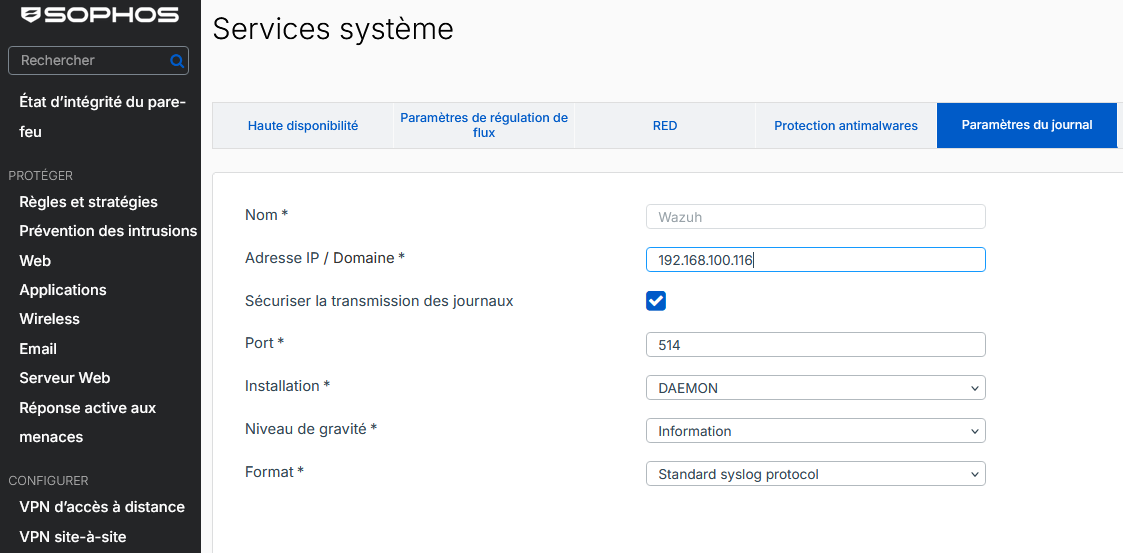
\includegraphics[width=0.9\textwidth]{images/sophos_log.png}
  \label{fig:sophos-log}
  \caption{Paramétrage d'envoi du journal Sophos}
\end{figure}
\par\bigskip
\subsubsection{Analyse}

Une fois les logs reçus par le serveur Wazuh, il faut analyser ces évenements. Pour ce faire, Wazuh utilise un fonctionnement en 3 étapes :

\begin{enumerate}
  \item[$\bullet$] Premièrement, on utilise une fonction de prematch pour filtrer les logs à considérer et à ignorer.
  \item[$\bullet$] Ensuite, Wazuh utilise des \textbf{décodeurs}. C'est décodeurs extraient les champs importants dse logs à l'aide de regex.
  \item[$\bullet$] Dernièrement, les champs extraits passent aux travers de \textbf{règles}. Ces règles définissent une ou plusieurs limites à ne pas dépasser, ainsi que le niveau de l'alerte à génerer.
\end{enumerate}

Nous allons voir ensemble un ajout de décodeurs et de règles pour détecter une connexion d'appareil non-autorisé sur le réseau Wifi.
\par\bigskip

Partons du log brut envoyé par le Gateway Unify pour une nouvelle connexion au réseau Wifi :\\
\begin{figure}[H]
  \centering
  \begin{minipage}{1\textwidth}
\begin{lstlisting}[]
E.....@.?.e...i...dt.f....{^<30>Jun 23 15:21:12 UNF-Gateway UNF-Gateway dnsmasq-dhcp[2715]: DHCPACK(br0) 192.168.106.181 52:fc:c1:5b:51:5e Redmi-Note-11-Pro
\end{lstlisting}
  \label{fig:raw-log}
  \caption{Exemple de log brut Unify - connexion établie}
  \end{minipage}
\end{figure}

Les champs intéressants sont les suivants :\\
\textbf{L'adresse MAC} de l'appareil qui s'est connecté, l'\textbf{adresse IP} qui lui a été attribué et le \textbf{hostname} qui permet humain d'identifier plus facilement l'appareil.\\
Faisons un décodeur pour extraire ces champs :

\begin{figure}[H]
  \lstinputlisting[language=XML, firstline=41, lastline=45]{Annexe/local-decoders.xml}
  \label{fig:unf-decoder}
  \caption{Décodeur de log de connexion au réseau Wifi}
\end{figure}
\par\bigskip

Ce décodeur nommé "\textbf{ubiquiti-dhcp-ack}", utilise le prematch "\textbf{dnsmasq-dhcp}" : Il ne considère que les logs où la chaine de caractères "\textbf{dnsmasq-dhcp}" est présente. De la même mainière, la chaine "\textbf{DHCPACK}" est présente en texte brut afin de ne considérer seulement l'évenement lorsque la connexion est établie et éviter de faux positifs.\\
\\
Afin de séparer les différents champs, nous utilisons une regex, les champs à extraire sont délimités par des parenthèses. Si des parenthèses sont présentes dan le log, elles pourront être matchées en échappant la parenthèse du regex avec un antislash.\\
Le champ \textbf{<order></order>} permet de nommer les champs extraits par regex afin de les réutiliser dans les règles.\\
Une fois l'évenement décodé, nous pouvons l'analyser à l'aide des règles suivantes :
\par\bigskip
\par\bigskip
\begin{figure}[H]
  \lstinputlisting[language=XML, firstline=33, lastline=47]{Annexe/local-rules.xml}
  \label{fig:unf-rules}
  \caption{Règles de connexion au réseau Wifi}
\end{figure}
\newpage
La structure basique d'une règle wazuh nous est exposée ci-dessus. Chaque règle a un \textbf{ID} unique, une \textbf{sévérité} entre 0 et 15, et une \textbf{description} de l'alerte qui sera générée, dans laquelle nous pouvons réutiliser les champs extraits par le décodeur.\\
Pour appliquer cette règle à la sortie du bon décodeur, on le déclare dans la balise \textbf{decoded\_as}. Il nous reste le plus important à detailler, la condition d'activation.\\
\\
Nous utilisons une liste \textbf{CDB}, c'est un fichier qui se présente sous forme de \textbf{clé:valeur} et qui nous permet de vérifier qu'une clé ou que l'association clé:valeur existe ou non dans ce fichier.\\
Pour ces règles, nous avons créé une liste de toutes les adresse MAC des équipements de Mesulog, qui sont donc autorisés à se connecter sur le réseau.
\par\bigskip
\begin{figure}[H]
  \centering
  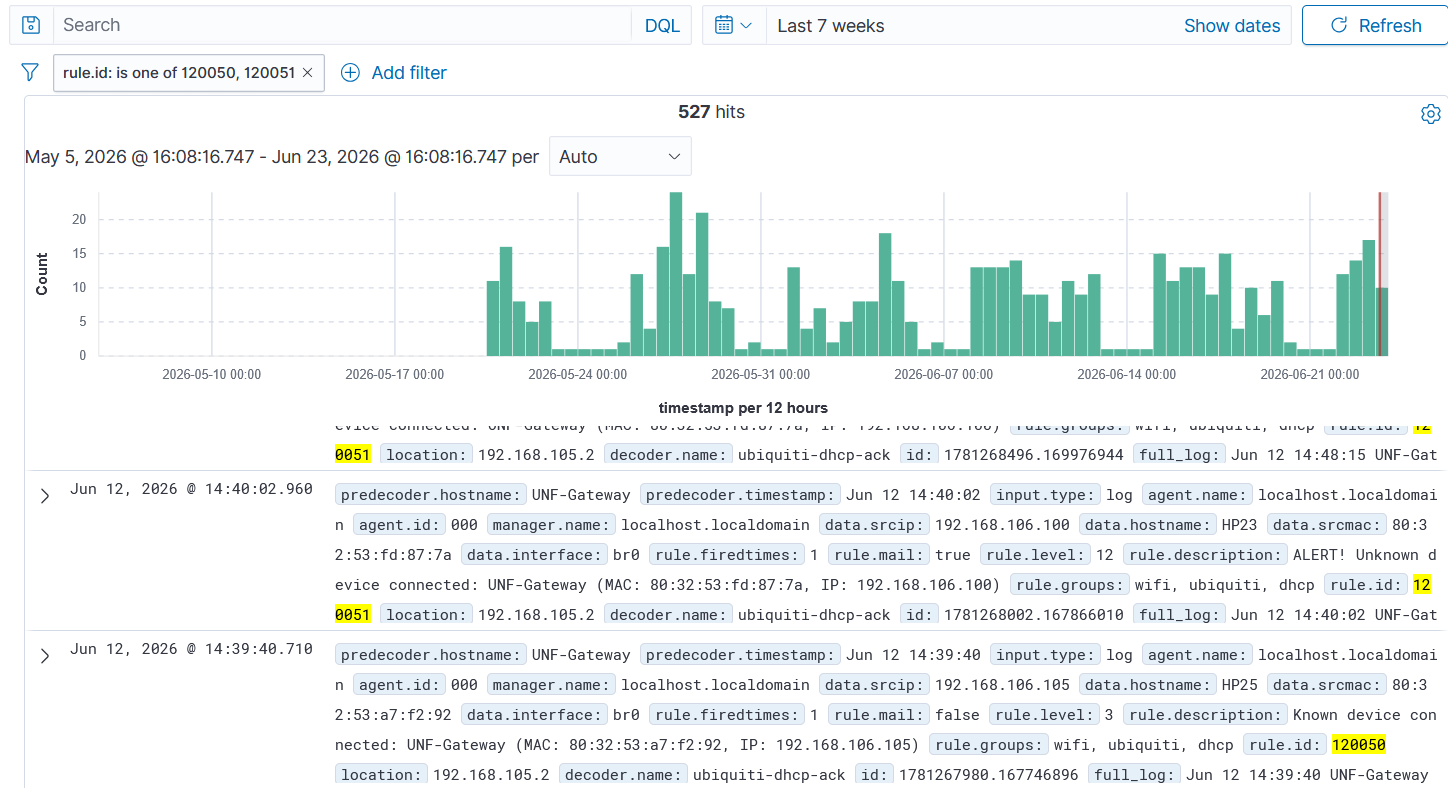
\includegraphics[width=1\textwidth]{images/discover-wazuh.png}
  \label{fig:discover-wazuh}
  \caption{Interface web de Wazuh regroupant les règles activées}
\end{figure}
\par\bigskip
Une fois que les règles sont déclenchées, il ne reste plus qu'a créer des alertes afin de prévenir les administrateurs système et réseau par mail.
\newpage
\subsubsection{Wazuh API}

Wazuh possède aussi une API, accessible par le web, qui nous permet d'interagir avec le serveur Wazuh depuis d'autres applications. j'ai pu utiliser cette API pour externaliser certains traitements de logs incommode sur Wazuh.\\
\\
L'ojectif principal d'analyser les journaux de logs du pare-fau Sophos était de détecter une fuite de donnée vers un tiers. Ainsi comme l'exemple précédent nous avons créé plusieurs décodeurs pour extraire le nombre d'octets de chaque trame loggée apr le Pare-feu. Cependant, il s'est avéré très compliqué de correctement détecter une fuite de donnée :\\
\\
En effet, pour mesurer un transfert de donnée de 1Go sur 1 heure, nous pourrions faire une première règle de niveau 0 (qui ne génere pas d'alerte) avec une limite d'octets arbitraire de 10Mo, puis une deuxième règle se déclanchant seulement si la première règle à été déclenchée 100 fois en une heure. La logique étant que 100 fois 10Mo fait 1Go.\\
Cependant, cette façon de faire (en utilisant les paramètres "frequency" et "timeframe" de Wazuh) n'est pas viable car il y a une infinité de multiplication possible pour atteindre une limite de 1Go. Dès lors, il est nécessaire d'externaliser ce traitement. Nous avons décider d'utiliser un script python pour automatiser ce processus.\\
\\
Ce scipt nommé "sophos-exfiltration.py" est présent sur la machine wazuh dans "/var/ossec/integrations". Etant donnée que ce script ne rentre pas sur une page entière, il est disponible en \hyperref[fig:sophos-integration]{Annexe}.\\
\\
Premièrement, nous récupérons un token d'authentification à l'API Wazuh avec les identifiants d'un utilisateur créé dans Wazuh pour ce programme. Ensuite, nous recherchons tous les évenements produits entre l'heure actuelle et un délai de temps définit, ici 1h avant ; les arguments de cette requête sotn encodés en json. Ensuite, nous regroupons ces données par adresse ip source et faisons la somme du nombre d'octets envoyés.\\
Il suffit maintenant de comparer ces sommes à la limite actuelle. Nous avons une limite de 1Gb de 8h à 19h les jours de la semaine et une limite de 100Mb la nuit(19h à 8h) et les weekends. Ainsi si cette limite est dépassée en 1h, une alerte est générée et insérée dans le fichier d'alerte de Wazuh.\\
\\
Pour que cette alerte se déclenche dans Wazuh, il faut l'ajouter dans un fichier de règle avec la forme :
\begin{figure}[H]
  \centering
  \lstinputlisting[language=XML, firstline=53, lastline=58]{Annexe/sophos-rules.xml}
  \label{fig:api-wazuh}
  \caption{Règle wazuh pour remonter l'alerte de l'intégration Python}
\end{figure}
\par\bigskip
Il est important de laisser le niveau de sévérité de cette règle à 0, car cette règle se déclenche si une alerte du même ID est active. L'alerte générée par le programme Python a déjà une sévérité qui primera sur une sévérité 0, mais la règle Wazuh pourrait se déclencher elle même en boucle si elle émettais une alerte. Une règle au niveau 0 ne déclenche pas d'alerte, empêchant cette réaction en chaine.
\newpage
\subsection{Durcissement du système d'information à l'aide des standards CIS}

L'une de mes missions principales a été de contribuer au durcissement du système d'information
 de l'entreprise en appliquant les recommandations du Center for Internet Security (CIS).

 \paragraph{Durcissement système}

 Le durcissement système est un ensemble de procédés de restriction des droits visant à réduire la surface d'attaque possible sur un système
 informatique, cette mission se concentre sur le durcissement d'ordinateurs Windows 11 via les les Group Policy Objects (GPO)
 mais le procédé de durcissement existe également sur les systèmes Linux. Il y a plusieurs façon de durcir des systèmes comme
 l'installation d'une image préconfiguré pour être durcie ou bien l'application de GPO suivant des standards prédéfinis.

\subsubsection{Les standards CIS}

  Plusieurs standards sont disponibles afin de durcir les systèmes windows, notemment:
  \begin{itemize}
    \item[$\bullet$] Microsoft Security Baselines
    \item[$\bullet$] CIS Benchmarks
    \item[$\bullet$] NIST Cybersecurity Framework
    \item[$\bullet$] STIGs (Security Technical Implementation Guides)
  \end{itemize}
\par\bigskip

  Le CIS propose des benchmarks de sécurité pour différents systèmes d'exploitation, applications et configurations,
   visant à réduire les vulnérabilités et à renforcer la résilience face aux attaques. Ces benchmarks sont organisés en 2 niveaux :
   \par\bigskip
  \begin{itemize}
    \item[$\bullet$] le Level 1 représente les configurations de sécurité essentielles et facilement déployables
    \item[$\bullet$] le Level 2 inclut des mesures plus restrictives adaptées aux environnements hautement sécurisés.
  \end{itemize}

  
  \par\bigskip
  
  Après évaluation des différents standards disponibles, nous avons décidé d'appliquer les standards CIS Level 1 sur l'ensemble de notre parc informatique.
  Ce choix a été motivé par le fait que les benchmarks CIS Level 1 sont déjà présents et intégrés dans le module Security Configuration Assessment (SCA) de Wazuh,
  permettant ainsi une détection et une validation automatisées des configurations de sécurité sans nécessiter des outils supplémentaires.

  \par\bigskip
  \paragraph{Alignement avec ISO 27001}

L'application des recommandations CIS Level 1 s'aligne naturellement avec
 les exigences de la norme ISO 27001. En effet, les baselines CIS contribuent au traitement des risques 
 et à la mise en œuvre de mesures techniques et organisationnelles correspondant aux contrôles 
 d'Annexe A par exemple la gestion des accès, exploitation sécurisée et protection des actifs ( A.9, A.12, A.8). 
 Cette approche facilite la démonstration de conformité lors d'un audit ISO 27001 en fournissant des preuves de
  configuration, de surveillance et d'amélioration continue des contrôles de sécurité.

 \newpage 
\subsubsection{Création d'un schéma structuré dans l'Active Directory}

Avant de déployer les configurations, la première étape était de créer un schéma structuré dans l'Active Directory (AD) afin de mieux hiérarchiser les comptes 
utilisateurs ainsi que les ordinateurs et serveurs présents sur le domaine. Cette structuration permet de faciliter la gestion 
des permissions, d'améliorer la visibilité sur les ressources et de renforcer la sécurité en limitant les accès aux ressources sensibles
 par le principe du moindre privilège.
\par\bigskip

Voici le schéma Active Directory initialement mis en place :\\


\begin{figure}[H]
\centering

\begin{tikzpicture}[
    every node/.style={draw, rounded corners, align=center},
    level 1/.style={sibling distance=8cm},
    level 2/.style={sibling distance=3cm},
    level distance=1.8cm
]

\node {mesulog.local}
    child { node {Computers}
        child { node {PC-01} }
        child { node {PC-02} }
        child { node {$\cdots$} }
    }
    child { node {Users}
        child { node {Alice} }
        child { node {Bob} }
        child { node {$\cdots$} }
    };

\end{tikzpicture}

\caption{Organisation initiale de l'Active Directory}
\end{figure}

Bien que ce schéma minimale soit fonctionnel, il ne permet pas de gérer efficacement les ressources et les permissions, il présente les défauts suivants :\\
\begin{itemize}
    \item[$\bullet$] Absence d'Unités d'Organisation (OU) pour regrouper les ressources par fonction, département ou niveau de sensibilité.
    \item[$\bullet$] Manque de groupes de sécurité pour attribuer des permissions de manière centralisée et éviter les permissions directes sur les comptes utilisateurs ou ordinateurs.
    \item[$\bullet$] Difficulté à appliquer des stratégies de groupe (GPO) spécifiques à certaines catégories d'utilisateurs ou d'ordinateurs en raison de l'absence de hiérarchie claire.
\end{itemize}
\par\bigskip


Afin de pallier à ces problèmes, il a été proposé et mis en place une nouvelle organisation de l'Active Directory, structurée autour de plusieurs OU et groupes de sécurité. Cette nouvelle organisation permet une gestion plus efficace des ressources, une meilleure application des politiques de sécurité et une réduction des risques liés à des permissions mal configurées.
Voici le schéma de l'Active Directory après restructuration :\\

\begin{figure}[H]
\centering
\resizebox{\textwidth}{!}{%
\begin{tikzpicture}[
    every node/.style={
        draw,
        rounded corners,
        align=center,
        font=\small
    }
]
% Niveau 0
\node (root) at (4,7) {mesulog.local};
% Niveau 1
\node (mesulog) at (4,5.5) {Mesulog};
% Niveau 2
\node (ord) at (-3.5,4) {Ordinateurs};
\node (usr) at (5,4) {Utilisateurs};
\node (svc) at (11,4) {Comptes de service};
% Niveau 3 - Ordinateurs
\node (postes)   at (-3.5,2.5) {Postes};
\node (serveurs) at (-6.5,2.5) {Serveurs};
% Niveau 3 - Utilisateurs
\node (admU) at (2.5,2.5)  {Administrateurs};
\node (devU) at (5,2.5)    {Développeurs};
\node (dirU) at (7,2.5)    {Direction};
\node (staU) at (9,2.5)    {Stagiaires};
% Niveau 4 - Postes
\node (admP) at (-6.5,1)   {Administrateurs};
\node (devP) at (-4,1)     {Développeurs};
\node (dirP) at (-2,1)     {Direction};
\node (staP) at (-0.2,1)   {Stagiaires};
% Connexions principales
\draw (root)   -- (mesulog);
\draw (mesulog) -- (ord);
\draw (mesulog) -- (usr);
\draw (mesulog) -- (svc);
\draw (ord) -- (serveurs);
% Connexions Ordinateurs
\draw (ord) -- (postes);
% Connexions Utilisateurs
\draw (usr) -- (admU);
\draw (usr) -- (devU);
\draw (usr) -- (dirU);
\draw (usr) -- (staU);
% Connexions Postes
\draw (postes) -- (admP);
\draw (postes) -- (devP);
\draw (postes) -- (dirP);
\draw (postes) -- (staP);
\end{tikzpicture}
}%
\caption{Organisation de l'Active Directory après restructuration}
\label{fig:ad-restructure}
\end{figure}

Le schéma ci-dessus représente l'organisation finale de l'Active Directory, son découpage est le suivant:
\par\bigskip


\begin{itemize}
  \item[$\bullet$] \textbf{Ordinateurs} composé de l'OU \textbf{Postes} réparties entre les \textbf{Administrateurs}, \textbf{Développeurs}, \textbf{Direction} et \textbf{Stagiaires} ainsi que de l'OU \textbf{Serveurs}
  \item[$\bullet$] \textbf{Utilisateurs} composé des différents utilisateurs du domaine également répartie entre les \textbf{Administrateurs}, \textbf{Développeurs}, \textbf{Direction} et \textbf{Stagiaires}
  \item[$\bullet$] \textbf{Comptes de services} composé des comptes utilisés par certains serveurs pour accéder à différentes machines et serveurs présents sur le domaine, le but est d'éviter d'utiliser un seul compte qui aurait trop de droits sur l'ensemble du domaine en définissant un compte par utilisation (e.g. compte de sauvegarde)
\end{itemize}
\par\bigskip

Ce découpage permet de mieux hiérachiser les droits selon les personnes dans l'entreprise, les développeurs bénéficient par exemple de plusieurs droits relatifs à la virtualisation afin
de développer dans des machines virtuelles, les autres fonctions de l'entreprises comme la Direction qui ne s'occupe que de document légaux et organisationelle ne bénéficient pas de ces droits car inutiles dans leurs cas.


\subsubsection{Stratégie de déploiement des GPO}
Afin de déployer les GPO de durcissement, il a été décidé de suivre une approche progressive, tout d'abord, l'ensemble des GPO
recommandées ont été réparties dans un classeur excel en fonction de :
\par\bigskip

\begin{itemize}
  \item[$\bullet$] leur nom
  \item[$\bullet$] leur description
  \item[$\bullet$] le numéro de la recommandation CIS correspondante
  \item[$\bullet$] leur impact potentiel sur les utilisateurs et les systèmes
  \item[$\bullet$] leur criticité, niveau de sécurité (faible, moyenne, élevée)
  \item[$\bullet$] leur pertinence par rapport aux besoins et au contexte de l'entreprise
  \item[$\bullet$] leur catégorie (gestion des comptes, sécurité réseau, protection des données, etc.)
  \item[$\bullet$] leur statut (À tester, Déployée, Exclue)
\end{itemize}
\par\bigskip
Cette classification a permis après une revue par l'ensemble de la DSI (Administrateurs Systèmes et RSSI) de prioriser les GPO les plus importantes avant de les déployer.
\par\bigskip
Le déploiement a lui été réparties en plusieurs itérations successives espacées dans le temps de plusieurs jours entre chaque, le but était de comprendre au plus vite
si une GPO ne fonctionnait pas par rapport à un cas d'utilisation non prévu lors de l'évaluation préliminaire.
\par\bigskip

Une convention de nommage fut également établie afin de faciliter la gestion et la maintenances des GPO, 
par exemple, la stratégie \textit{IT1* - Paramétrage des stratégies d'audits} est répartie selon les champs suivants :\\

\begin{table}[H]
\centering
\begin{tabular}{|c|p{10cm}|}
\hline
\textbf{Champ} & \textbf{Description} \\
\hline
IT1 & Numéro de l'itération durant laquelle la GPO a été créée ou déployée. \\
\hline
* & Indique que plusieurs GPO participent à une même fonctionnalité et sont regroupées logiquement. \\
\hline
Paramétrage des stratégies d'audit & Description concise de l'objectif ou du contenu de la GPO. Les termes utilisés peuvent être « Paramétrage », « Activation », « Désactivation », etc. selon la nature de la configuration appliquée. \\
\hline
\end{tabular}
\caption{Convention de nommage des GPO}
\end{table}

\subsubsection{Evolution de la conformité}

Tous les tests de conformités ont été réalisés à l'aide du module SCA de Wazuh sur le PC HP026
 situé dans l'OU "Postes\textbackslash Administrateurs" qui est un poste de travail utilisé par 
 les administrateurs systèmes de l'entreprise.\\ 
 À ce moment, les 4 premières itérations viennent d'être effectuées, le processus de choix et de revue étant particulièrement
 long, il se peut que l'on ne puisse avoisiner les 100\% de conformité avant la fin de l'alternance, cependant, 
 l'objectif est d'atteindre au moins 70\% de conformité sur ce poste. Ci-dessous se trouve la capture d'écran de Wazuh montrant le niveau de conformité du poste HP026 avant le début du déploiement des GPO :
\begin{figure}[H]
\centering
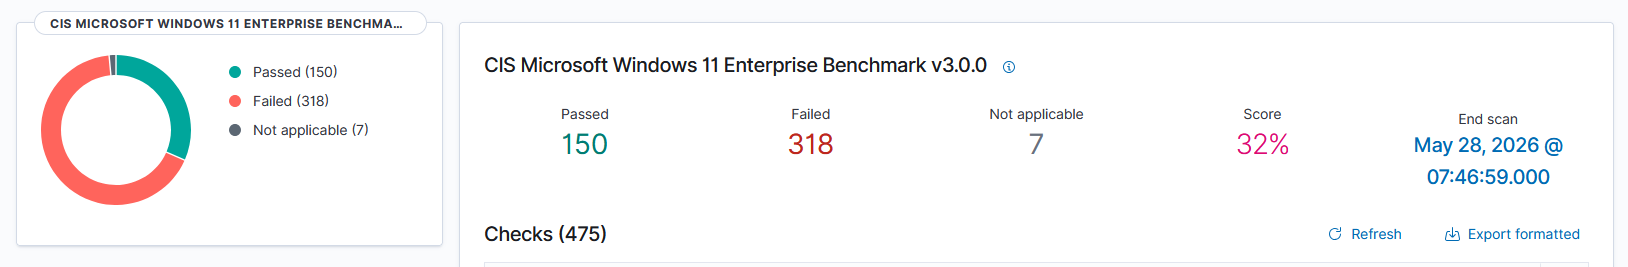
\includegraphics[width=0.8\textwidth]{images/wazuh-av-IT1.png}
\caption{Conformité du poste HP026 avant la première itération de déploiement des GPO}
\end{figure}


On observe que la conformité est faible, seulement 32\%, ce qui montre l'importance de cette mission de durcissement
 du système d'information.\\

Afin de visualiser la progression obtenue au fil des itérations, le graphique ci-dessous présente l'évolution
du taux de conformité aux standards CIS Level 1 pour le poste HP026, depuis l'état initial jusqu'à la quatrième
itération de déploiement des GPO.

\begin{figure}[H]
\centering
\begin{tikzpicture}
\begin{axis}[
  width=0.9\textwidth,
  height=0.45\textwidth,
  ymin=30,
  ymax=55,
  xmin=0,
  xmax=4,
  xtick={0,1,2,3,4},
  xticklabels={Commencement,Itération 1,Itération 2,Itération 3,Itération 4},
  ytick={30,35,40,45,50,55},
  ylabel={Conformité CIS Level 1 (\%)},
  xlabel={Itérations de déploiement},
  grid=both,
  line width=0.8pt,
  mark size=2.5pt
]
\addplot[
  color=blue,
  mark=* 
] coordinates {
  (0,32)
  (1,35)
  (2,41)
  (3,45)
  (4,49)
};
\end{axis}
\end{tikzpicture}
\caption{Évolution de la conformité CIS Level 1 du poste HP026 sur 4 itérations}
\end{figure}

Après l'itération 4, le taux de conformité a atteint 49\%, ce qui représente une amélioration
 significative par rapport à l'état initial de 32\%. Il reste cependant une marge de progression afin d'atteindre
  l'objectif de 70\% de conformité, ce qui nécessitera la poursuite du déploiement des GPO et l'ajustement des
   configurations en fonction des résultats obtenus lors des prochaines itérations.

\subsubsection{Exemples concrets de GPO appliquées}
Viser un objectif de conformité est intéressant seulement si on donne du sens à cet objectif, il est important
 de comprendre les différentes attaques ou vulnérabilités que l'on cherche à traiter en appliquant ces GPO,
  voici quelques exemples concrets de GPO appliquées et des attaques ou vulnérabilités qu'elles permettent de traiter :\\

\begin{table}[H]
\centering
\renewcommand{\arraystretch}{1.4}
\begin{tabular}{|p{1.5cm}|p{3cm}|p{5.2cm}|p{5.2cm}|}
\hline
\textbf{N° CIS} & \textbf{Nom} & \textbf{Objectif technique} & \textbf{Risque traité / Impact} \\
\hline
 26303 
  & Désactiver l'exécution automatique des médias 
  & Empêcher l'exécution automatique de code depuis supports amovibles (CD, USB, etc.). 
  & Empêche l'exécution de payloads malveillants déposés sur des médias amovibles (autorun/autoplay). Faible impact pour postes standards, peut gêner certains usages nomades. Déployé en pilote. \\
\hline
 26028 
  & Désactiver le cache des ouvertures de session précédentes 
  & Ne pas stocker localement les informations des sessions précédentes (cache d'identifiants/jetons). 
  & Réduit l'impact en cas de vol ou compromission d'un poste (réutilisation de sessions/cookies). Moyennement contraignant pour utilisateurs nomades~; à tester avant déploiement large. \\
\hline
 26193 
  & Désactiver le protocole LLMNR 
  & Désactiver LLMNR/mDNS sur les interfaces afin d'empêcher la résolution de noms non sécurisée. 
  & Évite les attaques de type LLMNR/NBT-NS poisoning permettant le détournement de trafic et le vol d'identifiants. Recommandé en environnement d'entreprise~; faible impact fonctionnel si DNS interne est bien configuré. \\
\hline
\end{tabular}
\caption{Exemples concrets de GPO appliquées et des risques associés}
\end{table}
\subsubsection{Limitation du module SCA de Wazuh}

Bien que pratique, le module SCA de Wazuh n'en reste pas moins limité, voici comment il fonctionne :\\

\begin{enumerate}
  \item Pour chaque ordinateur / Serveur, un fichier \textit{.xml} avec des commandes pour tester l'application des GPO est envoyé dessus
  \item Ces commandes présentes dans le fichier sont ensuite exécutées par un script sur les machines
  \item Le résultat de ce script est ensuite envoyé à Wazuh Manager afin d'être traité et de calculer le taux de conformité.
\end{enumerate}


\par\bigskip
\paragraph{Le problème de conformité}


Nous avons constaté après l'application de plusieurs GPO que le taux de conformité n'augmentait pas malgré le fait que les GPO soient appliquées sur les machines,
 après investigation, il s'est avéré que le module SCA ne prenait pas en compte certaines configurations appliquées par les GPO,
  ce qui faussait le taux de conformité affiché dans Wazuh.\\

  En ouvrant le fichier \textit{xml} envoyé par Wazuh sur les machines nous avons constaté que quand le module SCA testait 
  l'application d'une GPO, il vérifiait la configuration d'une clé de registre spécifique, cependant, certaines GPO appliquaient des configurations qui n'étaient pas liées à des clés de registre,
 pour ces dernières, le module test directemment de la conformité d'un paramètre via une commande PowerShell, voici une exemple concret:

\begin{figure}[H]
  \centering
  \begin{minipage}{\textwidth}
\begin{lstlisting}[language=ScaYAML]
- id: 26145
  title: "Ensure 'Audit Credential Validation' is set to 'Success and Failure'."
  description: "This subcategory reports the results of validation
      tests on credentials submitted for a user account logon request."
  rationale: "Auditing these events may be useful when investigating
      a security incident."
  remediation: "To establish the recommended configuration via GP, [...] Validation"
  compliance:
    - cis: ["17.1.1"]
    - cis_csc: ["8.5"]
  condition: all
  rules:
    - 'c:auditpol.exe /get /subcategory:"Credential Validation"
        -> r:Success and Failure'
\end{lstlisting}
  \caption{Exemple d'un test SCA pour vérifier l'application d'une GPO}
  \label{fig12}
  \end{minipage}
\end{figure}


L'extrait ci-dessus représente un des tests présent dans le fichier \textit{xml} utilisé pour les tests de conformité Windows 11, il est utilisé pour vérifier que la stratégie d'audit "Audit Credential Validation" servant à créer des journaux 
d'audit lors de la validation des identifiants est bien configuré pour auditer à la fois les succès et les échecs.
\par\bigskip
Le champ rules contient la commande éxecuté après la chaine \textit{c:} et le résultat attendu après la chaine \textit{r:},
 si le résultat de la commande correspond au résultat attendu, alors le test est considéré comme réussi, sinon, il est considéré comme échoué.
\par\bigskip

 Lors de la deuxième itération, après le déploiement des GPO, nous avons constaté que le taux de conformité n'augmentait pas malgré le fait que les GPO soient appliquées,
 Curieux, nous avons d'abord vérifié que les ordinateurs récupéraient bien les nouvelles GPO:

\begin{figure}[H]
\centering
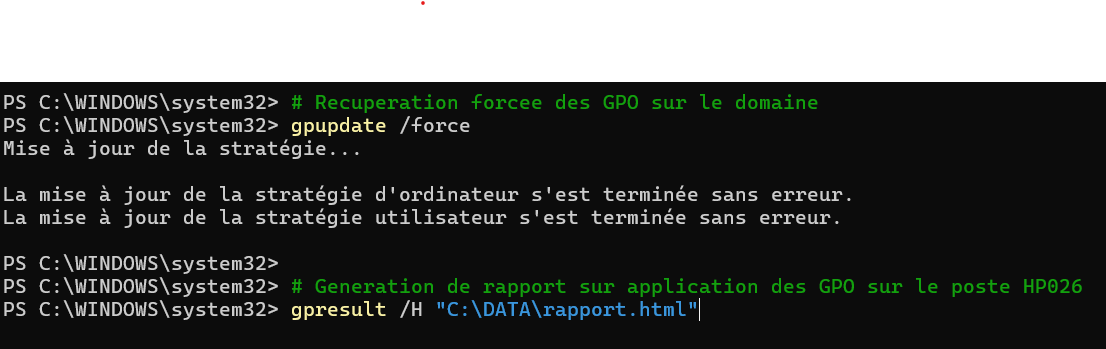
\includegraphics[width=0.8\textwidth]{images/RecupGPOEtGenerationRapport.png}
\caption{Commande gpupdate pour forcer la récupération des GPO sur le poste HP026}
\end{figure}


Une fois le rapport généré, nous avons constaté que les GPO étaient bien actives sur le poste :

\begin{figure}[H]
\centering
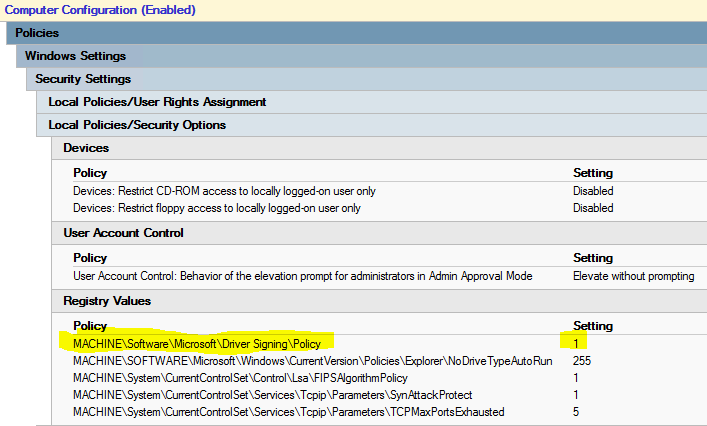
\includegraphics[width=0.7\textwidth]{images/gpReport.png}
\caption{Rapport d'application des GPO sur le poste HP026}
\end{figure}

Les GPO attendus apparaissants dans le rapport, nous avons donc décidé de vérifier directemment les commandes utilisées par le module SCA pour tester la conformité des GPO:

\begin{figure}[H]
\centering
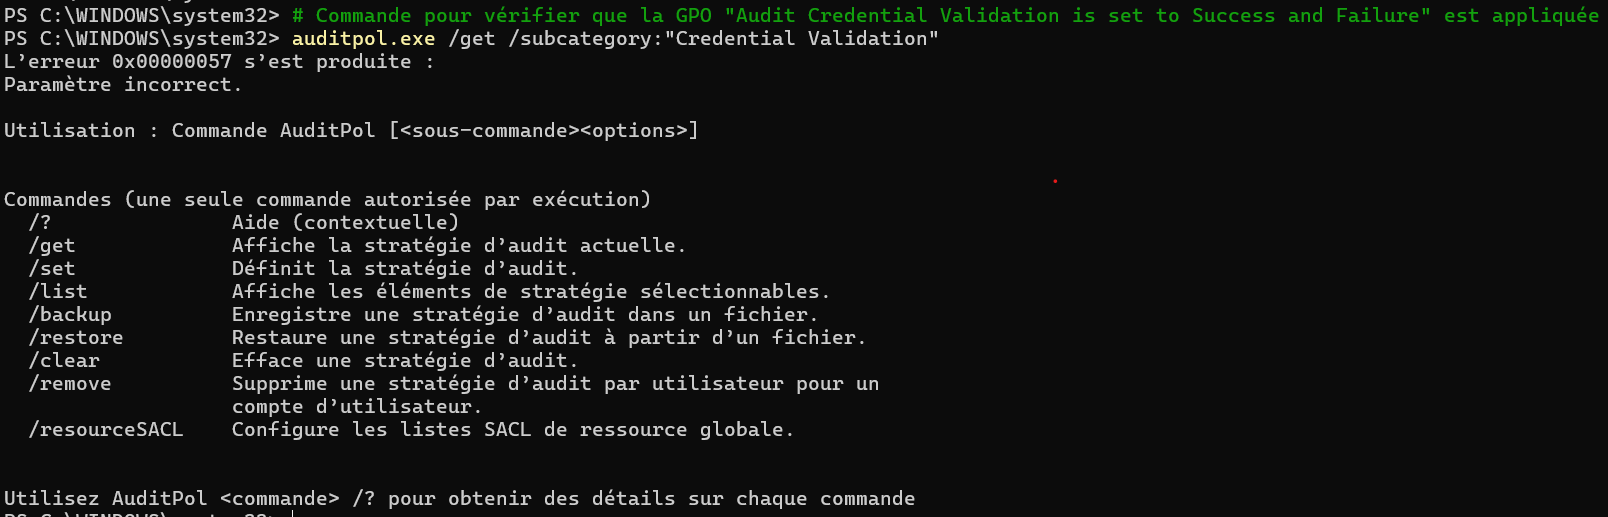
\includegraphics[width=1\textwidth]{images/auditcrd.png}
\caption{Rapport d'application des GPO sur le poste HP026}
\end{figure}

L'éxecution de cette commande a révélé plusieurs difonctionnemments:
\par\bigskip


\begin{itemize}
  \item[$\bullet$] Le nom de la GPO a vérifier n'était pas correctement écrit, il fallait soit appeler la GPO par son GUID soit par son nom exact dans la langue du système d'exploitation, dans notre cas, le nom de la GPO était "Validation des informations d'identification" au lieu de "Credential Validation"
  \item[$\bullet$] Le retour de la commande n'était pas correctement traité, le module SCA attendait le retour "Success and Failure" alors que la commande retournait "Succès et échec" à cause de la langue du système d'exploitation.
\end{itemize}

\paragraph{Solution}

Afin de remédier à ce problème, il a été décidé de modifier les commandes utilisées par
 le module afin d'inclure le GUID à la place du nom anglais ainsi que les résultats attendus en utilisant le résultat en français pour ce dernier.
 Cette modification a été réalisé sur l'ensemble du fichier lorsqu'une commande était utilisée pour vérifier l'application d'une GPO.
\par\bigskip

L'utilisation des accents dans la langue française a elle posé un autre souci, en effet l'agent
 Wazuh exécutent les commandes via PowerShell en tant qu'agisseur système, ce qui limite le support UTF-8 natif. 
 Pour contourner ce problème, nous avons encapsulé la commande \texttt{auditpol} dans une commande PowerShell avec l'encoding UTF-8, 
 permettant ainsi d'utiliser directement les caractères accentués comme "Succès et échec". La commande suivante a été implémentée :

\begin{figure}[H]
\centering
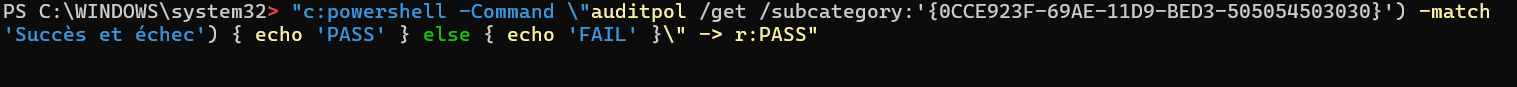
\includegraphics[width=1\textwidth]{images/commande_qui_passe.png}
\caption{Commande PowerShell modifiée pour supporter les accents}
\end{figure}

Une fois ce problème reglé, nous avons eu besoin de déployer le nouveau fichier de test sur l'ensemble des postes afin de recalculer le taux de conformité,
initialement, nous pensions que remplacer le fichier sur le serveur Wazuh Manager sous /var/ossec/test/sca et le supprimer des postes suffirait,
 cependant, après plusieurs tests, nous avons constaté que les agents ne récupéraient pas automatiquement le nouveau fichier de test.
 \par\bigskip

 Nous avons donc décidé de déployer le nouveau fichier sur les machines du parc via GPO, pour cela:
 \begin{itemize}
  \item 
 \end{itemize}

 [présenter la GPO de déploiement du fichier de test SCA sur les postes]


\subsubsection{Conclusion de la mission et critiques}

\paragraph{Axe d'amélioration possible - BloodHound}

BloodHound est un outil utilisé en Blue Team ou en Red Team, il permet d'analyser de la sécurité
 des réseaux Active Directory en représentant sous la forme de graphes les relations entre les utilisateurs,
  les groupes, les ordinateurs aini que les permissions au sein d'un domaine.\\
 En utilisant BloodHound, il est possible d'identifier les chemins d'attaque potentiels,
  les comptes à privilèges élevés et les vulnérabilités dans la configuration de l'Active Directory.
  \par\bigskip

  L'utilisation de BloodHound pourrait être un axe d'amélioration afin de renforcer davantage la sécurité de l'Active Directory
   en identifiant les chemins d'attaque potentiels et en mettant en place des mesures pour les atténuer.
    Par exemple, BloodHound pourrait révéler des comptes avec des permissions excessives ou des relations d'accès non sécurisées,
     permettant ainsi de les corriger avant qu'elles ne soient exploitées par des attaquants.

  [inclure un exemple]



\subsection{Création et implémentation d'une stratégie de sauvegarde}
\subsection{Entretien du parc informatique et missions annexes}

à ajouter en fonction de ce que je veux développer.

\begin{enumerate}
  \item debug du problème de synchronisation de l'Active Directory
  \item debug du problème de synchronisation de mail
  \item Diagnostique d'un problème de connexion au serveur nas
  \item installation de suricata
  \item configuration d'un réseau wifi invité
\end{enumerate}



\newpage
\section{Impact environnemental et sociétal}

\subsection{Impact de mes déplacements au long de mon alternance}

\subsubsection{Déplacements quotidiens}

Dans le cadre de mon alternance, j'effectuais un trajet domicile-travail aller-retour chaque jour ouvré. Les émissions de CO\textsubscript{2} ont été estimées à l'aide du calculateur de l'ADEME.\\

Le trajet quotidien se décompose comme suit :\\

\begin{itemize}
\item[$\bullet$] \textbf{Tramway} : 1,5 km, soit 0,03 g CO\textsubscript{2}e/km ;
\item[$\bullet$] \textbf{TER Grenoble -- Moirans} : 19 km, soit 0,17 g CO\textsubscript{2}e/km ;
\item[$\bullet$] \textbf{Marche à pied jusqu'au bureau} : 1,1 km, impact négligeable.
\end{itemize}
\par\bigskip

L'ensemble du trajet représente environ 3,68 g de CO\textsubscript{2}e par déplacement, soit 7,36 g de CO\textsubscript{2}e par journée de travail.\\

Sur une période estimée à 30 semaines d'alternance à raison de 5 jours par semaine, les déplacements domicile-travail représentent environ 1,1 kg de CO\textsubscript{2}e émis.

\subsubsection{Déplacements ponctuels}

Au cours de mon alternance, j'ai été amené à effectuer plusieurs déplacements professionnels, notamment vers le site de Nerys à Gardanne (Bouches-du-Rhône).\\

Ce trajet a été réalisé en covoiturage à trois personnes à bord d'un véhicule hybride de type SUV. La distance parcourue était d'environ 294 km pour un aller simple, soit 588 km aller-retour.\\

D'après les estimations réalisées à l'aide du calculateur de l'ADEME, ce déplacement représente environ 11,9 kg de CO\textsubscript{2}e pour l'aller-retour.\\

Bien que cette valeur soit significativement supérieure aux émissions générées par mes trajets quotidiens, ce type de déplacement est resté exceptionnel durant la période d'alternance.



\subsection{Actions écologiques et sociales des actions menées par l'entreprise}


\subsection{Impacts sociétaux des projets réalisés}





% -----------------------
% BILAN
% -----------------------
\section{Bilan personnel}


[justification de AC 33.1 et 33.03 du PN + AC 36.1 +36.03]\\

Cette alternance m’a permis de consolider et d’approfondir des compétences techniques en administration système, cybersécurité opérationnelle et développement, tout en les appliquant dans un contexte industriel réel et exigeant. Les missions confiées m’ont confronté à des problématiques concrètes de sécurisation du système d’information, de conformité réglementaire et de maintien en condition opérationnelle, dépassant largement le cadre théorique des enseignements.
\vspace{\baselineskip}
Le travail autour de l’homologation d’un système d’information « Diffusion Restreinte » a été particulièrement formateur. Il m’a permis de mieux appréhender les enjeux liés à la protection de données sensibles, à la formalisation des procédures de sécurité et à la rigueur nécessaire dans un contexte soumis à des exigences normatives fortes. Cette mission m’a également sensibilisé à l’importance de la documentation et de la traçabilité dans les démarches de cybersécurité.\vspace{\baselineskip}


Les projets liés au durcissement du système d’information, à la supervision de la sécurité via Wazuh et à la migration de l’Active Directory m’ont permis de développer une vision globale de l’infrastructure et de ses interdépendances. J’ai gagné en capacité d’analyse, en autonomie et en méthode, notamment dans la priorisation des actions de sécurité, l’analyse des vulnérabilités et la mise en œuvre de solutions adaptées aux contraintes de l’entreprise.
\vspace{\baselineskip}

Sur le plan humain et organisationnel, cette alternance m’a permis de m’intégrer au sein d’une équipe technique pluridisciplinaire, de participer aux échanges collectifs et de travailler en collaboration avec des profils variés. Les réunions de suivi et le travail en environnement professionnel m’ont aidé à améliorer ma communication technique et à structurer davantage ma démarche de travail.
\vspace{\baselineskip}

Cette expérience confirme mon intérêt pour les métiers de l’administration système et de la cybersécurité. Elle m’a permis de mieux définir mon projet professionnel, orienté vers la sécurisation et l’exploitation d’infrastructures informatiques, et constitue une étape déterminante dans la construction de mes compétences et de mon parcours professionnel.
\newpage
\section{Annexe}
%setup sql
\paragraph{Requêtes de nettoyages}
\begin{figure}[H]
  \lstinputlisting[language=SQL, firstline=1, lastline=53]{Annexe/Setup_query.sql}
  \caption{Requêtes de nettoyage des données -1ère partie}
  \label{fig:setup-access}
\end{figure}
\par\bigskip
\begin{figure}[H]
  \lstinputlisting[language=SQL, firstline=54, lastline=105]{Annexe/Setup_query.sql}
  \caption{Requêtes de nettoyage des données -2ème partie}
  \label{fig:setup-access-2}
\end{figure}
\par\bigskip
\begin{figure}[H]
  \lstinputlisting[language=SQL, firstline=106, lastline=155]{Annexe/Setup_query.sql}
  \caption{Requêtes de nettoyage des données -3ème partie}
  \label{fig:setup-access-3}
\end{figure}
\par\bigskip
\begin{figure}[H]
  \lstinputlisting[language=SQL, firstline=156, lastline=183]{Annexe/Setup_query.sql}
  \caption{Requêtes de nettoyage des données -4ème partie}
  \label{fig:setup-access-4}
\end{figure}

%extraction sql
\paragraph{Requêtes d'extractions}
\begin{figure}[H]
  \lstinputlisting[language=SQL, firstline=1, lastline=63]{Annexe/BANC_MOD_extraction_query.sql}
  \caption{Requêtes d'extraction de données -1ere partie}
  \label{fig:extraction-access}
\end{figure}
\par\bigskip
\begin{figure}[H]
  \lstinputlisting[language=SQL, firstline=64, lastline=125]{Annexe/BANC_MOD_extraction_query.sql}
  \caption{Requêtes d'extraction de données -2eme partie}
  \label{fig:extraction-access-2}
\end{figure}
\par\bigskip
\begin{figure}[H]
  \lstinputlisting[language=SQL, firstline=126, lastline=184]{Annexe/BANC_MOD_extraction_query.sql}
  \caption{Requêtes d'extraction de données -3eme partie}
  \label{fig:extraction-access-3}
\end{figure}
\par\bigskip
\begin{figure}[H]
  \lstinputlisting[language=SQL, firstline=186, lastline=213]{Annexe/BANC_MOD_extraction_query.sql}
  \caption{Requêtes d'extraction de données -4eme partie}
  \label{fig:extraction-access-4}
\end{figure}
\par\bigskip
\begin{figure}[H]
  \lstinputlisting[language=SQL, firstline=214, lastline=267]{Annexe/BANC_MOD_extraction_query.sql}
  \caption{Requêtes d'extraction de données -5eme partie}
  \label{fig:extraction-access-5}
\end{figure}
\par\bigskip
\begin{figure}[H]
  \lstinputlisting[language=SQL, firstline=268, lastline=310]{Annexe/BANC_MOD_extraction_query.sql}
  \caption{Requêtes d'extraction de données -6eme partie}
  \label{fig:extraction-access-6}
\end{figure}
\par\bigskip
\begin{figure}[H]
  \lstinputlisting[language=SQL, firstline=312, lastline=353]{Annexe/BANC_MOD_extraction_query.sql}
  \caption{Requêtes d'extraction de données -6eme partie}
  \label{fig:extraction-access-6}
\end{figure}
\par\bigskip7\begin{figure}[H]
  \lstinputlisting[language=SQL, firstline=355, lastline=394]{Annexe/BANC_MOD_extraction_query.sql}
  \caption{Requêtes d'extraction de données -7eme partie}
  \label{fig:extraction-access-7}
\end{figure}
\par\bigskip
\begin{figure}[H]
  \lstinputlisting[language=SQL, firstline=396, lastline=447]{Annexe/BANC_MOD_extraction_query.sql}
  \caption{Requêtes d'extraction de données -8eme partie}
  \label{fig:extraction-access-8}
\end{figure}
\par\bigskip
\begin{figure}[H]
  \lstinputlisting[language=SQL, firstline=448, lastline=465]{Annexe/BANC_MOD_extraction_query.sql}
  \caption{Requêtes d'extraction de données -9eme partie}
  \label{fig:extraction-access-9}
\end{figure}
\par\bigskip

%reste
\begin{figure}[H]
    \centering
    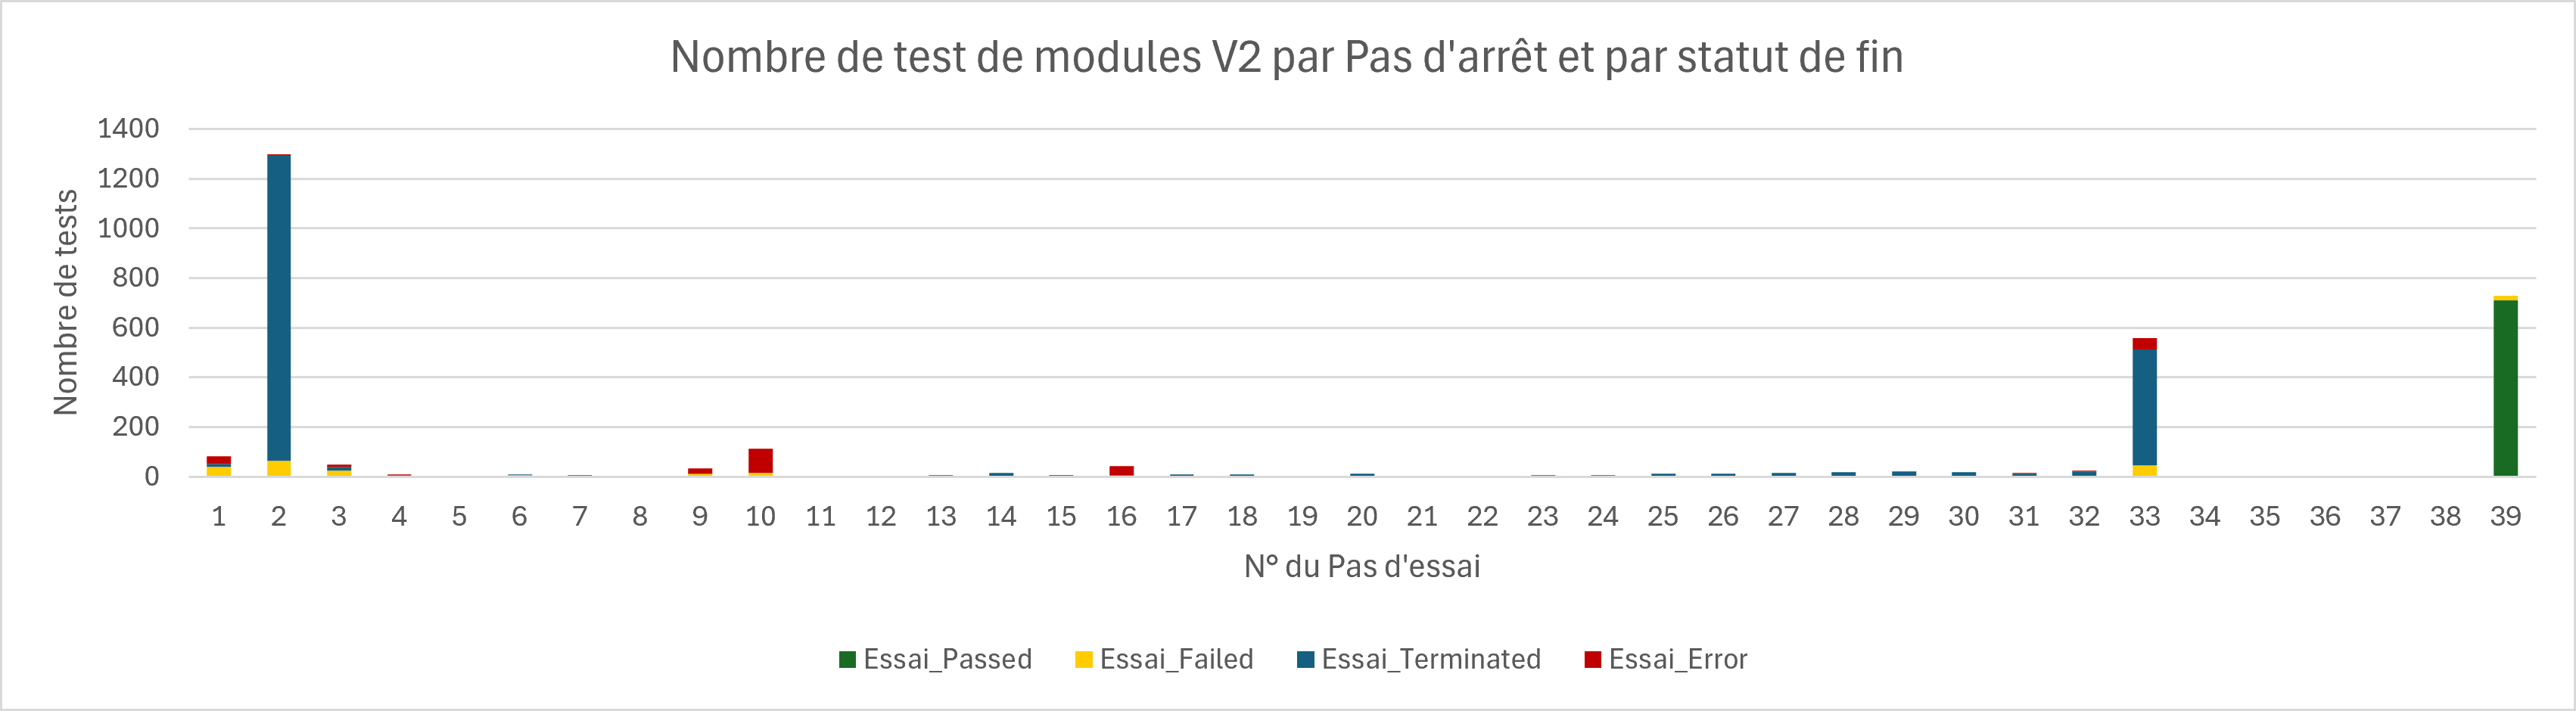
\includegraphics[width=1\textwidth]{images/nb_test_mod2_stepcount.png}
  \caption{Distribution des statuts de fin des essais par étape de l'essai, modules V2}
  \label{fig:graphiques}
\end{figure}
\par\bigskip
\begin{figure}[H]
    \centering
    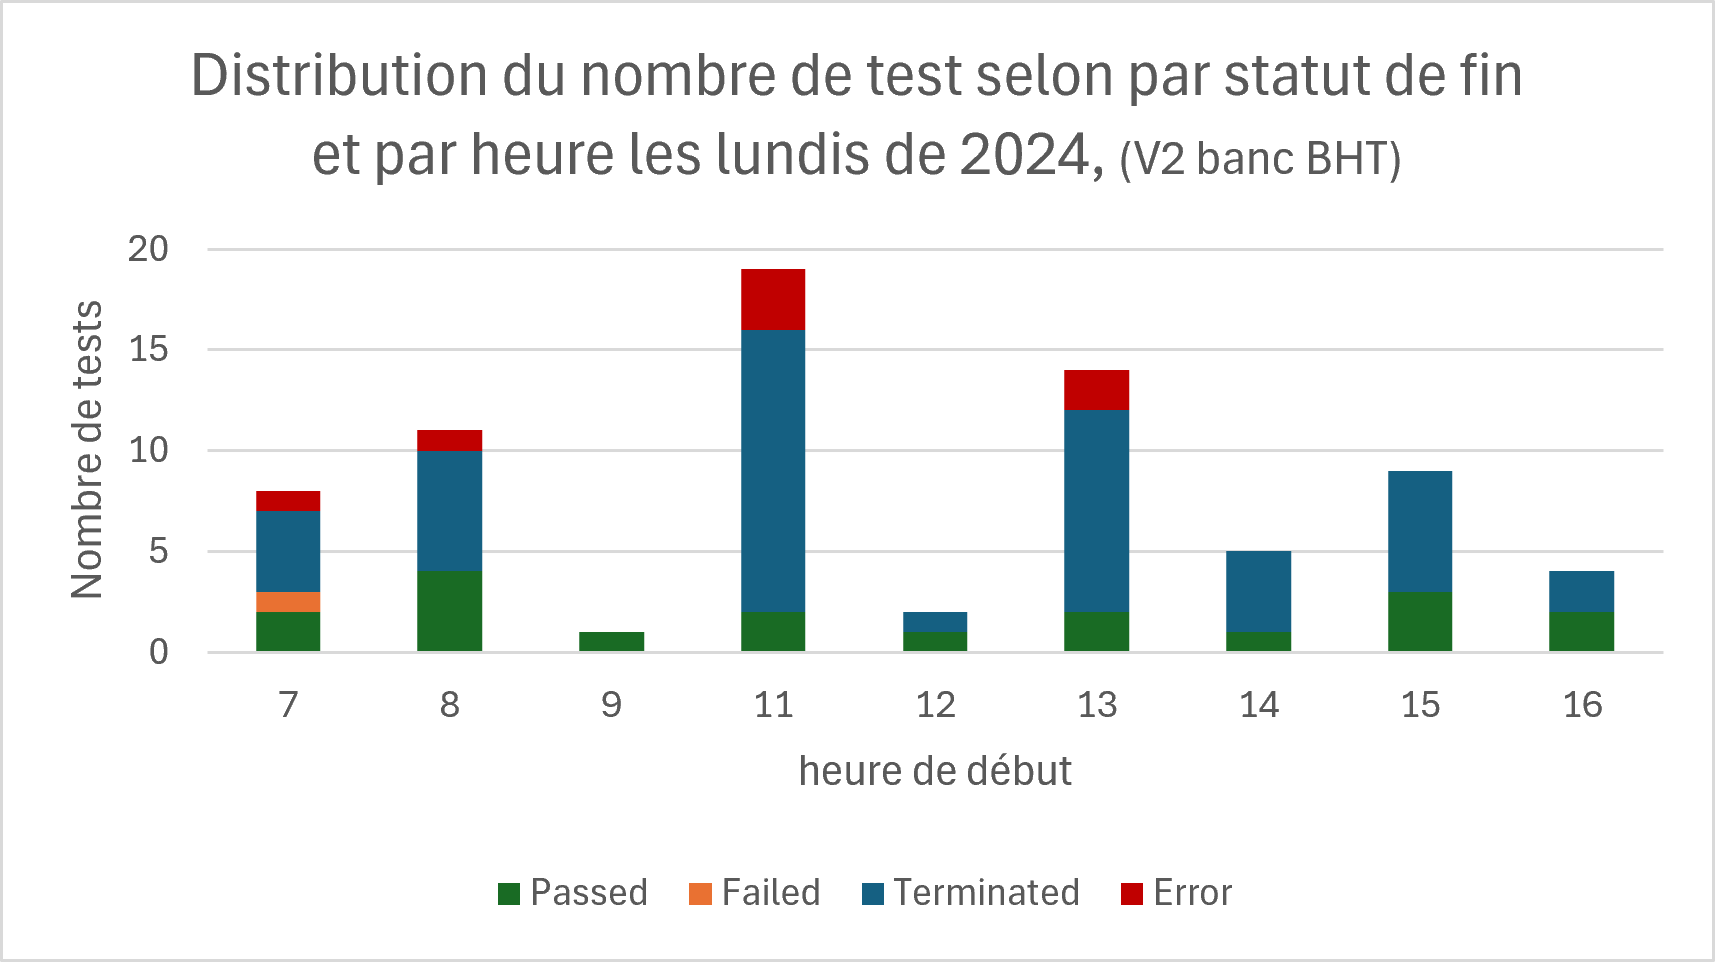
\includegraphics[width=1\textwidth]{images/nb_test_status_lundi-2024-V2-BHT.png}
  \label{fig:graph-lundi2024-bht}
\end{figure}
\par\bigskip
\begin{figure}[H]
    \centering
    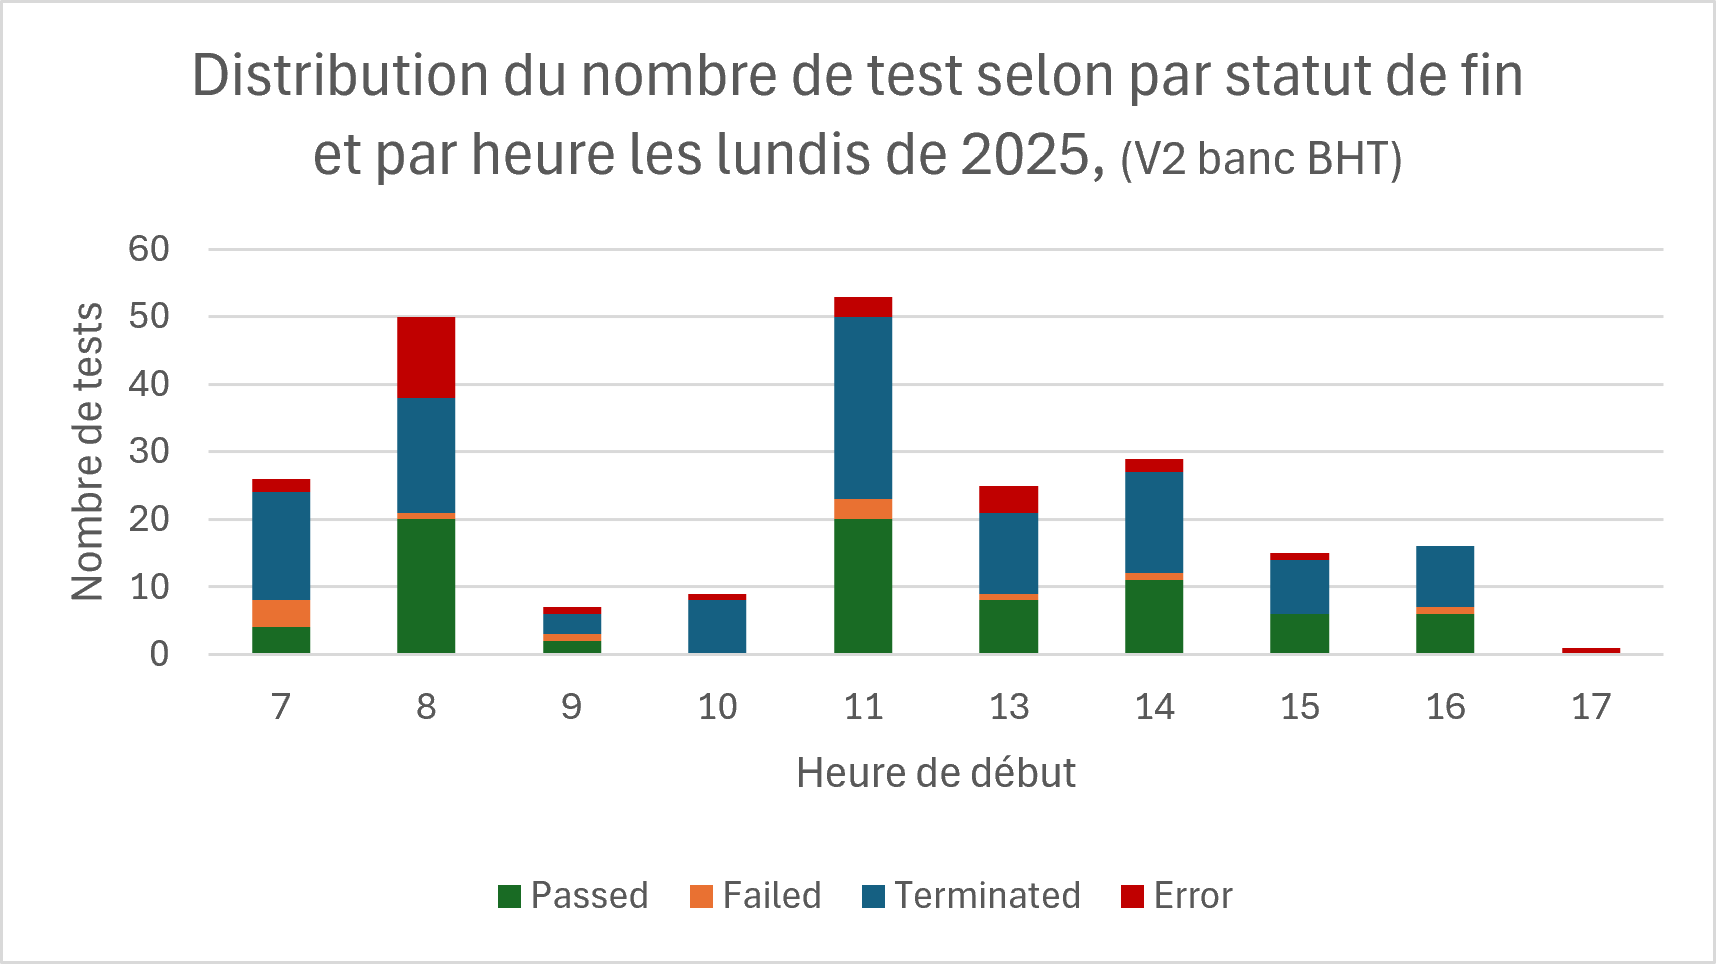
\includegraphics[width=1\textwidth]{images/nb-test-status-lundi-2025-V2-BHT.png}
  \label{fig:graph-lundi2025-bht}
\end{figure}
\par\bigskip
\begin{figure}[H]
    \centering
    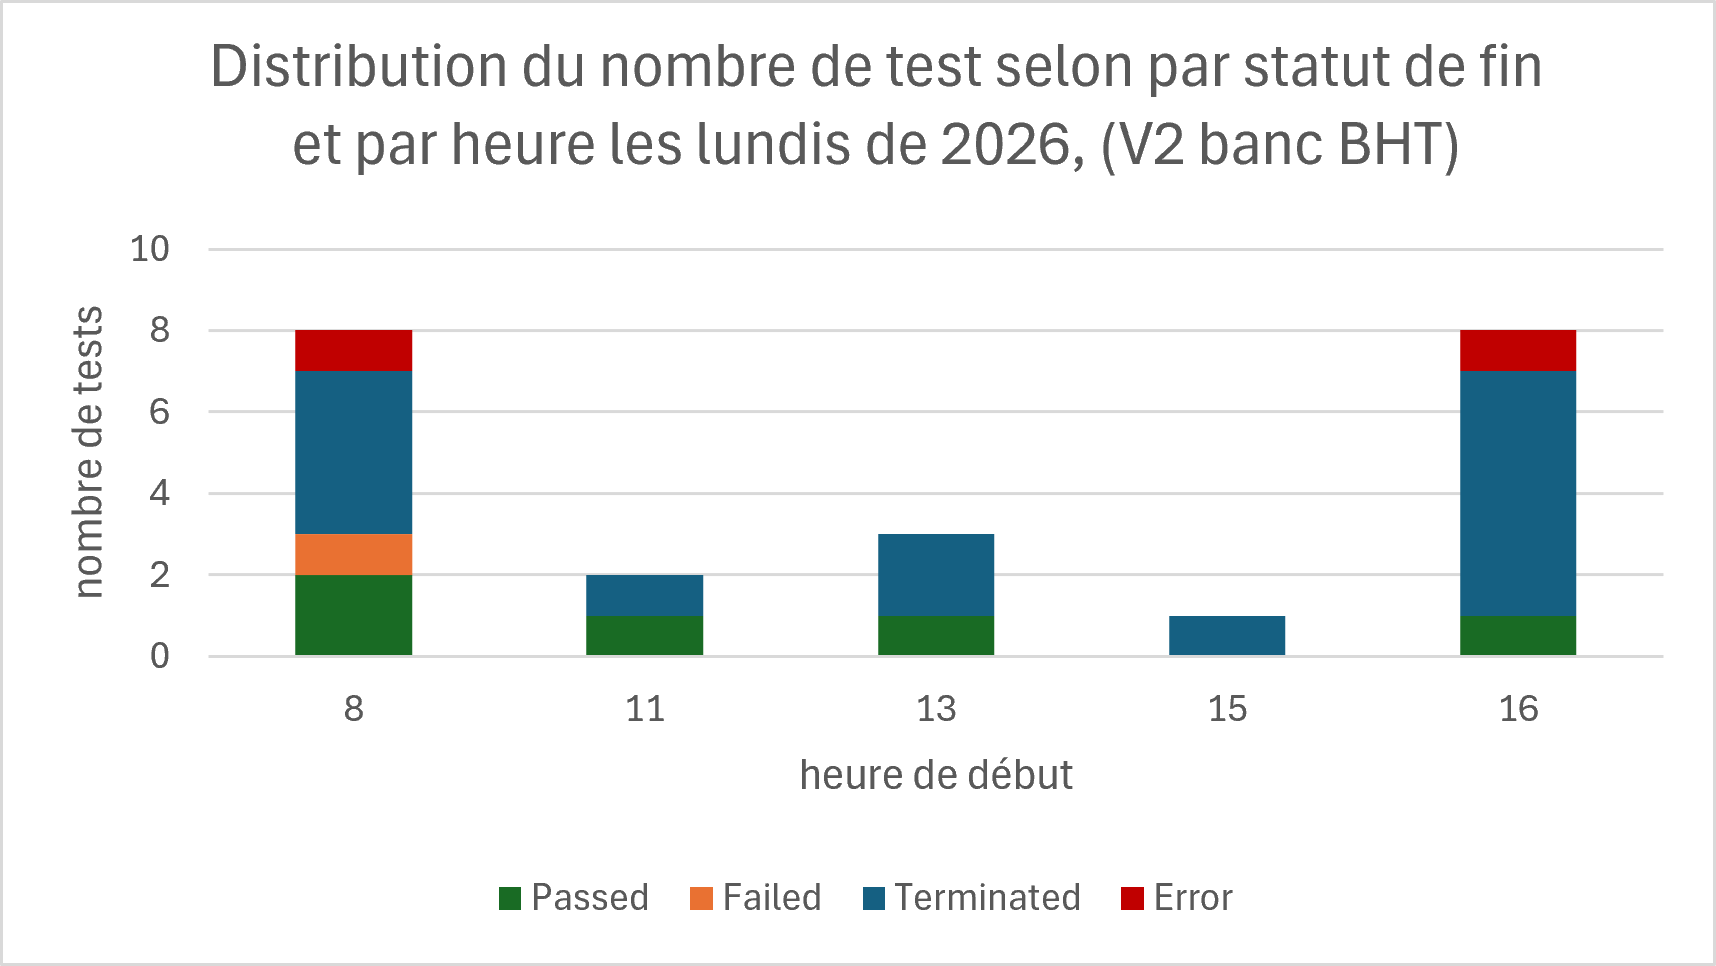
\includegraphics[width=1\textwidth]{images/nb-test-status-lundi-2026-V2-BHT.png}
  \label{fig:graph-lundi2026-bht}
\end{figure}
\begin{figure}[H]
    \centering
    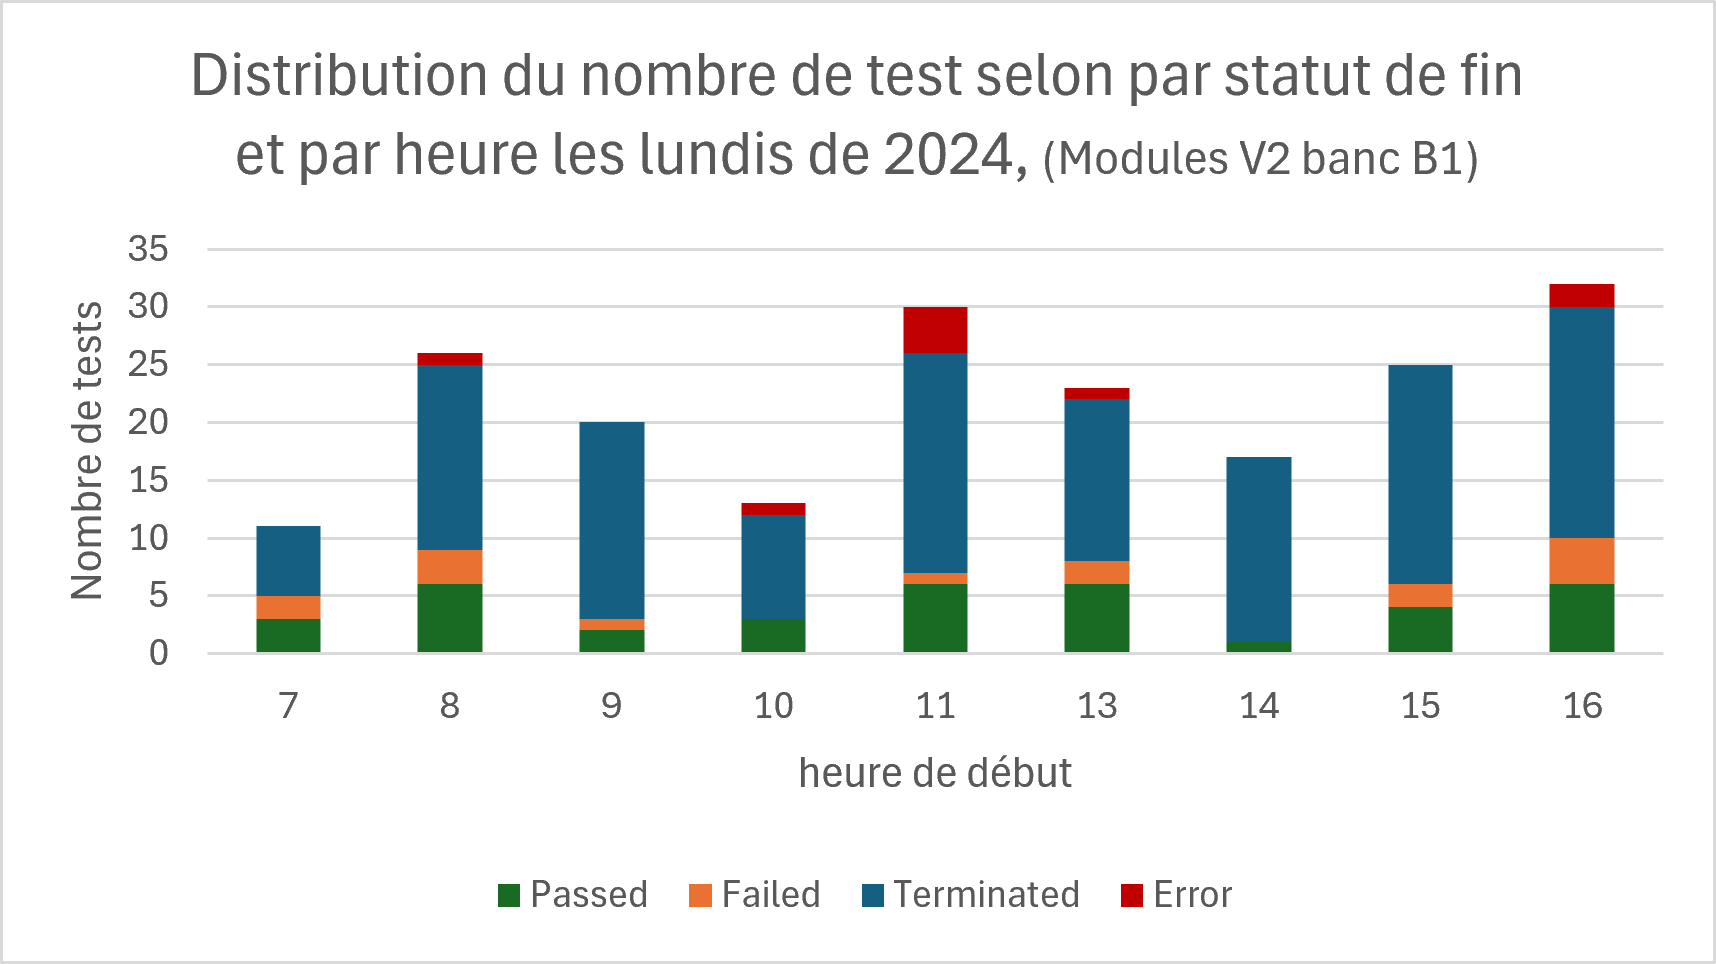
\includegraphics[width=1\textwidth]{images/nb-test-status-lundi-2024-V2-B1.png}
  \label{fig:graph-lundi2024-b1}
\end{figure}
\par\bigskip
\begin{figure}[H]
    \centering
    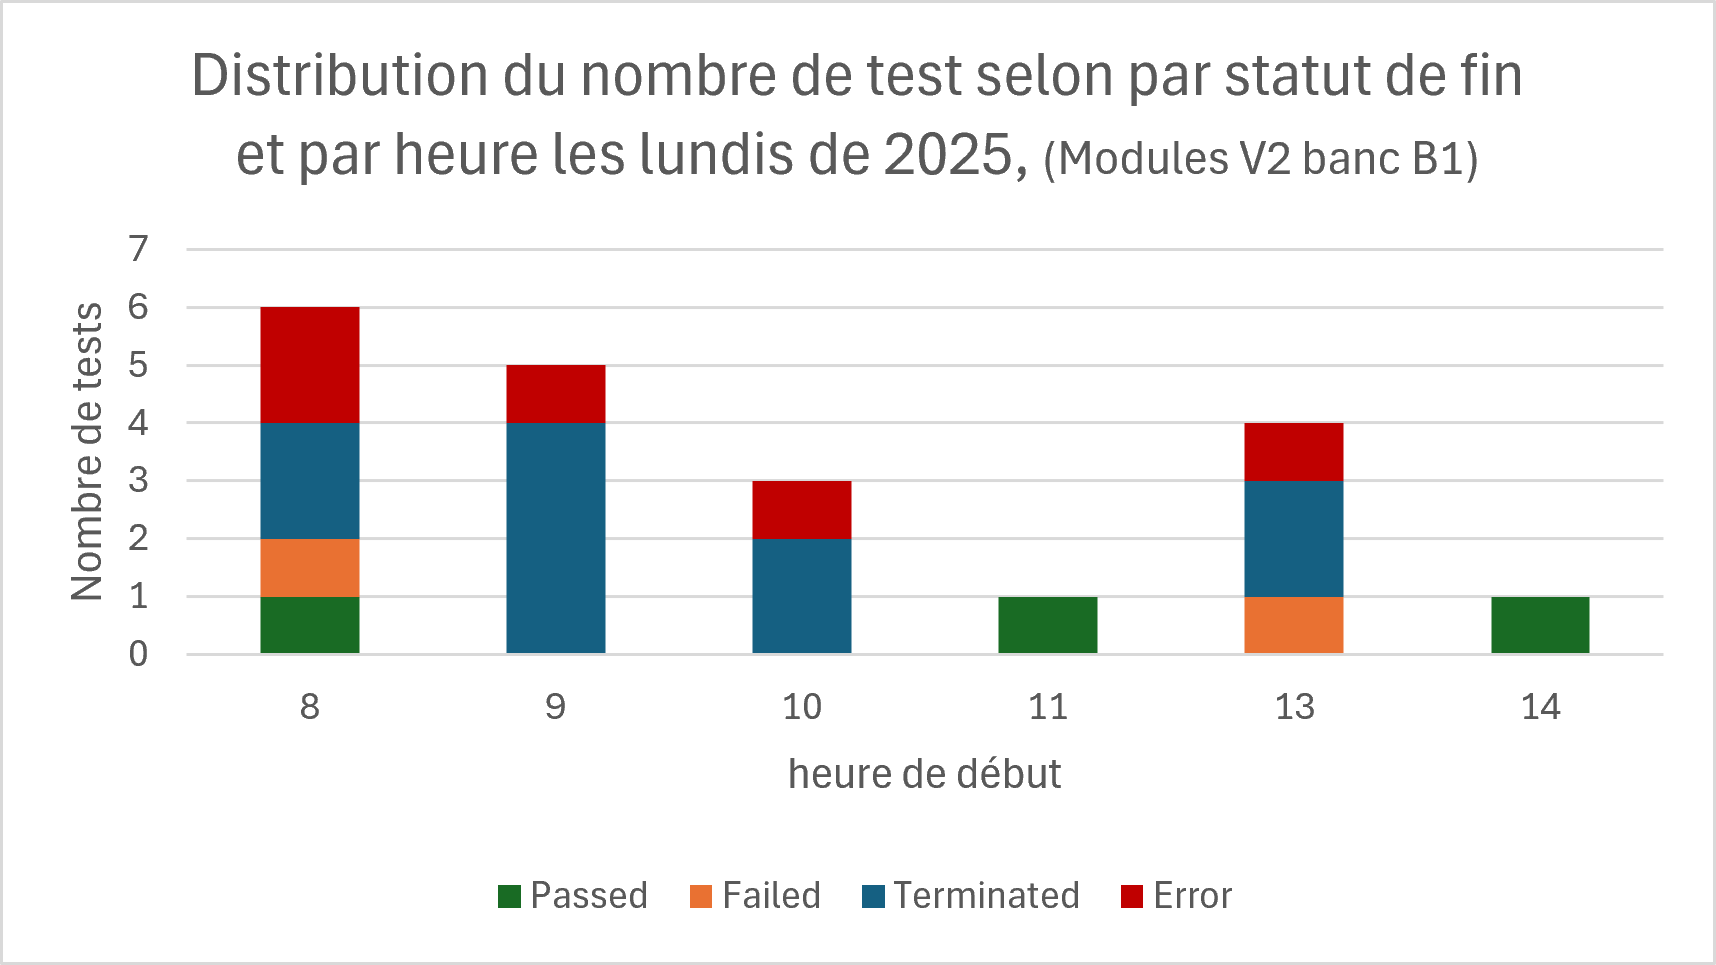
\includegraphics[width=1\textwidth]{images/nb-test-status-lundi-2025-V2-B1.png}
  \label{fig:graph-lundi2025-b1}
\end{figure}
\par\bigskip
\begin{figure}[H]
    \centering
    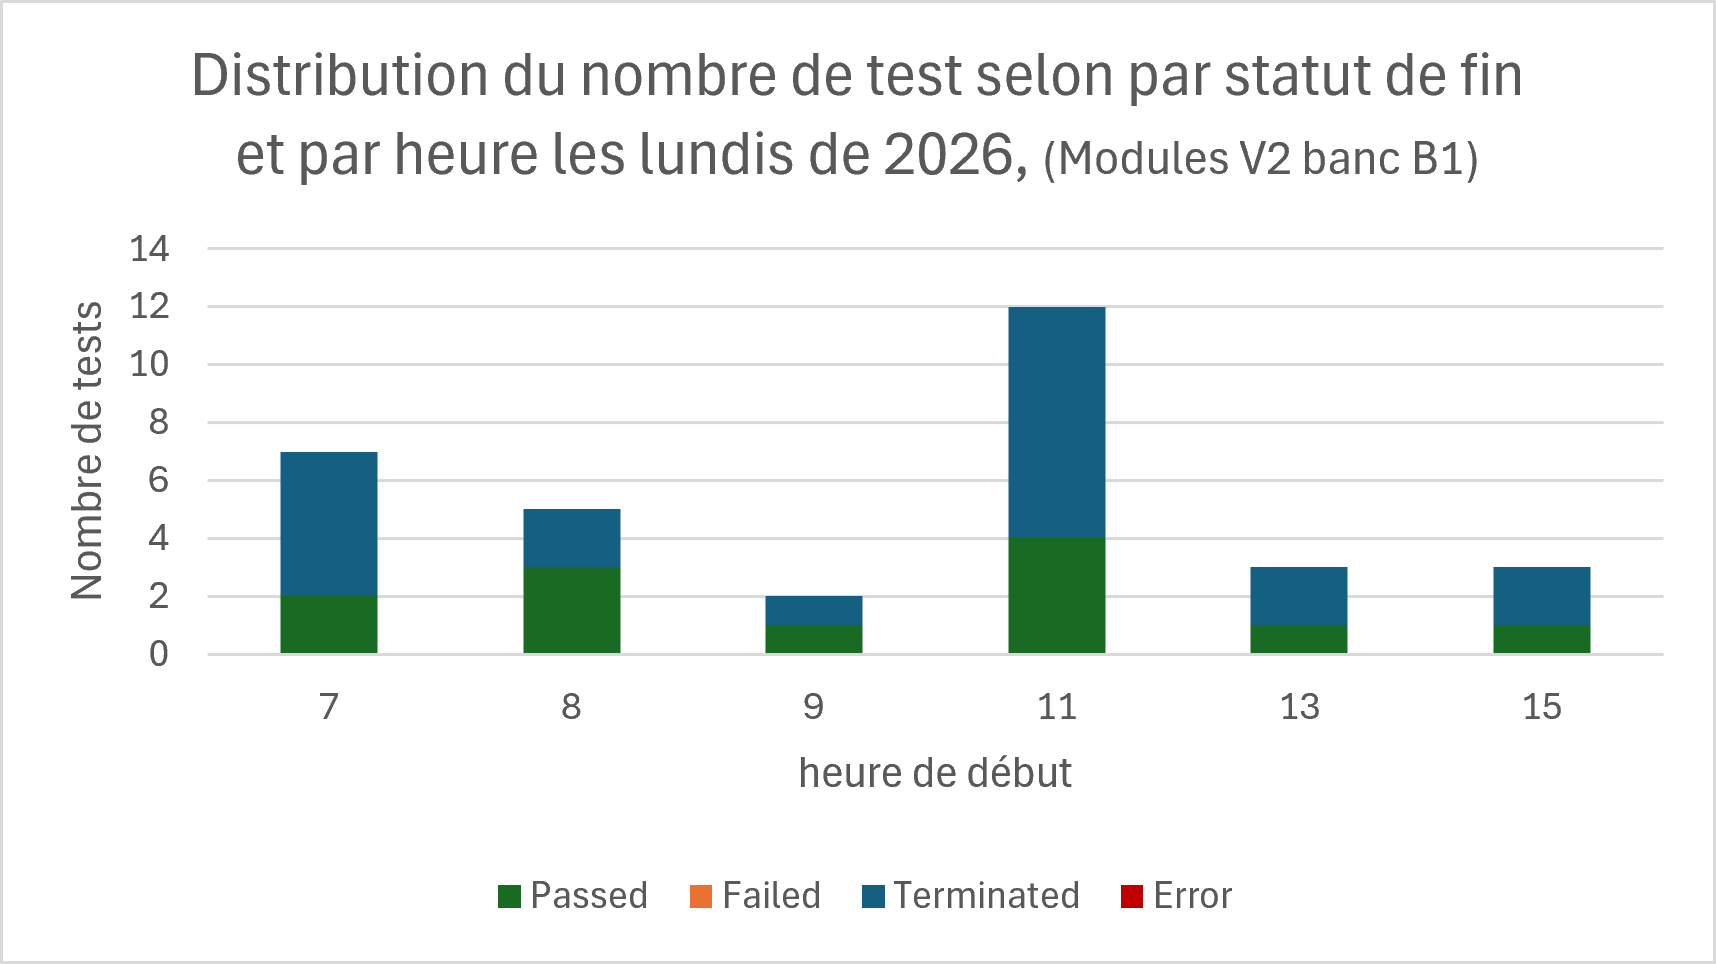
\includegraphics[width=1\textwidth]{images/nb-test-status-lundi-2026-V2-B1.png}
  \label{fig:graph-lundi2026-b1}
\end{figure}
\par\bigskip
%sophos integration.py
\begin{figure}[H]
  \lstinputlisting[language=Python, firstline=1, lastline=41]{Annexe/sophos-integration.py}
  \caption{Script sophos-exfiltration.py -1ere partie}
  \label{fig:sophos-integration}
\end{figure}
\par\bigskip
\begin{figure}[H]
  \lstinputlisting[language=Python, firstline=42, lastline=80]{Annexe/sophos-integration.py}
  \caption{Script sophos-exfiltration.py -2ème partie}
  \label{fig:sophos-integration-2}
\end{figure}
\par\bigskip
\begin{figure}[H]
  \lstinputlisting[language=Python, firstline=81, lastline=123]{Annexe/sophos-integration.py}
  \caption{Script sophos-exfiltration.py -3eme partie}
  \label{fig:sophos-integration-3}
\end{figure}
\par\bigskip
\begin{figure}[H]
  \lstinputlisting[language=Python, firstline=124, lastline=165]{Annexe/sophos-integration.py}
  \caption{Script sophos-exfiltration.py -4eme partie}
  \label{fig:sophos-integration-4}
\end{figure}
\par\bigskip
% -----------------------
% GLOSSAIRE
% -----------------------
\newpage
\printglossaries
\printnoidxglossary

% -----------------------
% BIBLIOGRAPHIE
% -----------------------
\paragraph{Références bibliographiques}
\addcontentsline{toc}{section}{Références}
 \begin{thebibliography}{moi}
\bibitem{[1]} ANSSI, \textit{OASIS — Recommandations pour les architectures des systèmes d’information sensibles ou Diffusion Restreinte}, ANSSI-PG-075 version 1.2, 24/09/2021.
\bibitem{[2]} ANSSI, \textit{Directive II 901-1 — Sécurisation des systèmes d’information sensibles}, Agence nationale de la sécurité des systèmes d’information, version en vigueur, 28/01/2015
\bibitem{[3]} Center for Internet Security (CIS), \textit{CIS Benchmarks}, https://www.cisecurity.org/cis-benchmarks/, consulté en 2024.
\bibitem{[4]} Microsoft, \textit{Active Directory Documentation}, https://docs.microsoft.com/en-us/windows-server/identity/active-directory-domain-services, consulté en 2024.
\bibitem{[5]} Wazuh, \textit{Wazuh Documentation}, https://documentation.wazuh.com/, consulté en 2024.
\end{thebibliography}
% -----------------------
% FIN DOCUMENT
% -----------------------
\end{document}